\chapter{Results}
The models of the previous sections are tested on \emph{trans}-polyacetylene. Since \emph{trans}-polyacetylene\footnote{In the following always \emph{trans}-polyacetylene is meant when only polyacetylene is said.} has an alternation of single and double bonds between the carbon atoms, a unit cell containing two CH-groups with periodic boundary conditions in one dimension is used (see \cref{image_scheme_polyacetylene_unit_cell}). 

\section{Convergence Tests for Polyacetylene}
\begin{figure}[]
	\centering
	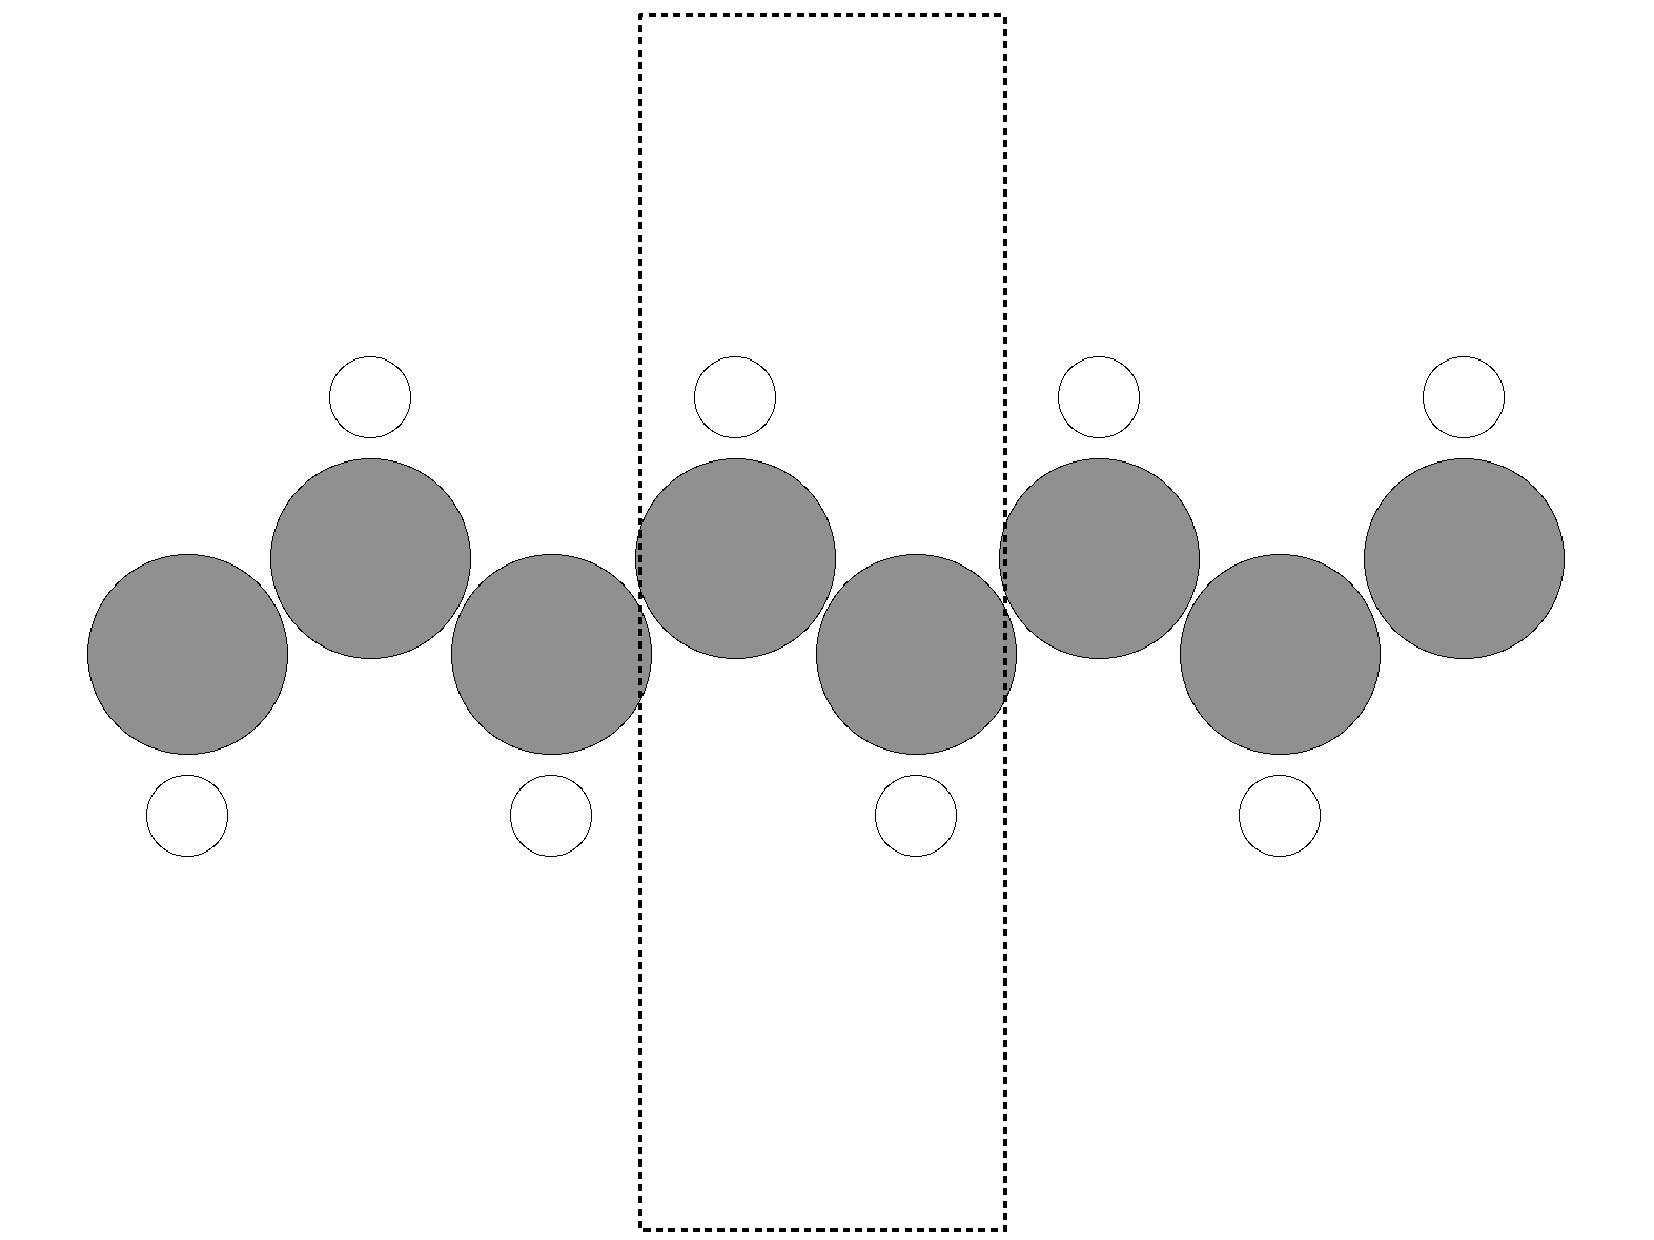
\includegraphics[width = .5\textwidth]{Images/polyacetylene/convergence/polyacetylene_nice_unit_cell}
	\caption{Scheme: Unit cell for \emph{trans}-polyacetylene with periodic boundary conditions in one dimension. The grey circles represent the carbon atoms, the white ones the hydrogen atoms.}
	\label{image_scheme_polyacetylene_unit_cell}
\end{figure}
To check the convergence in respect to a certain parameter, all other parameters are chosen in a way, that the energy is definitely converged in respect to them.\\
First the convergence of the ground state energy in respect to the number of used $k$- points is tested, whereat automatic \textsc{Brillouin} zone sampling is used. It can be seen that the energy is converged for approximately 15 $k$-points (see \cref{image_poly_kpts_energy}). Hence, a comparison of the energies for $15$ and $100$ $k$-points gives a difference of only $\unit[0.014]{eV}$.\\
In \cref{image_poly_grid_energy} the ground state energy in respect to the grid spacing $h$ can be seen. Since the number of grid points increases with $\nicefrac{1}{h^3}$, it is important to find a reasonable compromise between computing time and accuracy. Because the discussed system isn't that big, $h = \unit[0.1]{\AA}$ is used for further calculations.\\
The lowering of the ground state energy in respect to the maximum force for the relaxation process of the cores is small in comparison with previous dependencies (see \cref{image_poly_force_energy}). Therefore a maximum force of $\unitfrac[0.1]{eV}{\AA}$ should be appropriate.\\
Finally the convergence of the energy in respect to the unit cell width (not in the direction of the periodic boundary condition) is tested. As can be seen in \cref{image_poly_width_energy}, the ground state energy increases for small unit cell widths, which can be understood intuitively by comparison to the quantum mechanical 'particle in a box'. For a width of approximately $\unit[9]{\AA}$ a stable level is reached, which corresponds with a minimal distance between cores and cell surface of approximately $\unit[3]{\AA}$ (same for second direction of non periodic boundaries).\\
Convergence tests for other systems is done analogously and thus added to the appendix (see \cref{section_conv_hyd}).

\begin{figure}[]
	\centering
	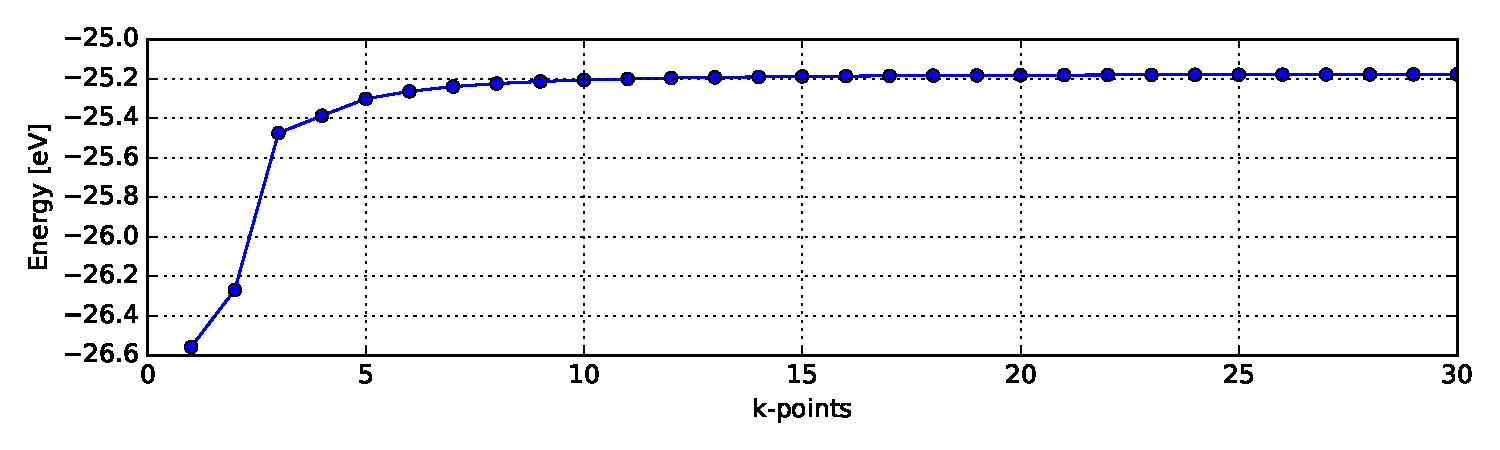
\includegraphics[width = 13cm]{Images/polyacetylene/convergence/kpts-energy}
	\caption{Ground state energy of relaxed polyacetylene in respect to the number of $k$-points.}
	\label{image_poly_kpts_energy}
\end{figure}
\begin{figure}[]
	\centering
	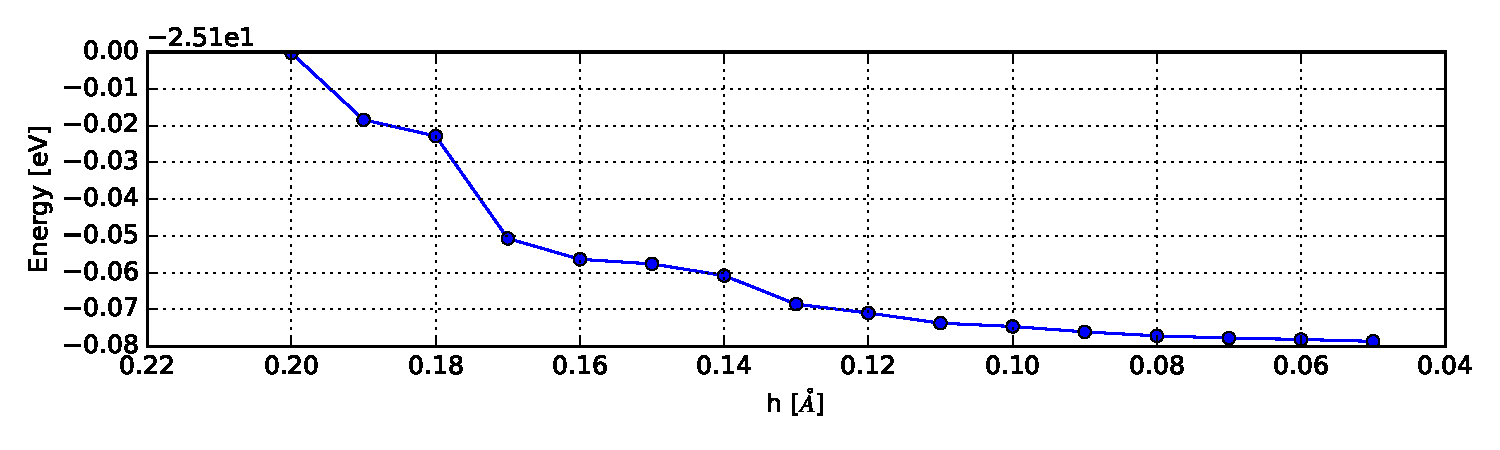
\includegraphics[width = 13cm]{Images/polyacetylene/convergence/gridspacing-energy}
	\caption{Ground state energy of relaxed polyacetylene in respect to the grid spacing.}
	\label{image_poly_grid_energy}
\end{figure}
\begin{figure}[]
	\centering
	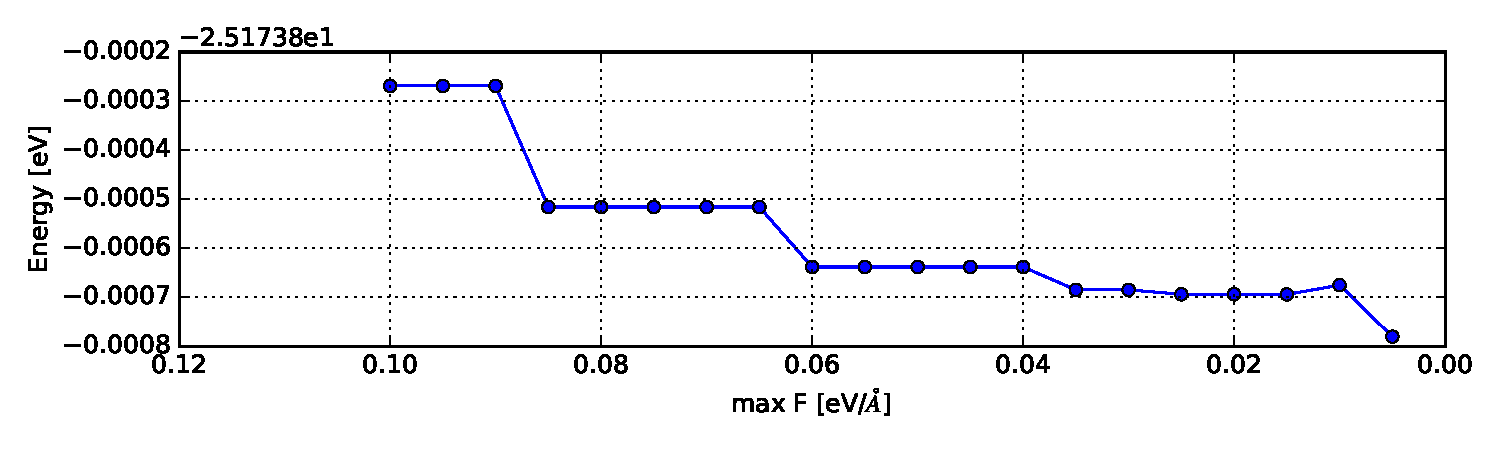
\includegraphics[width = 13cm]{Images/polyacetylene/convergence/forces-energy}
	\caption{Ground state energy of relaxed polyacetylene in respect to the maximum force, for which the relaxation process stops.}
	\label{image_poly_force_energy}
\end{figure}
\begin{figure}[]
	\centering
	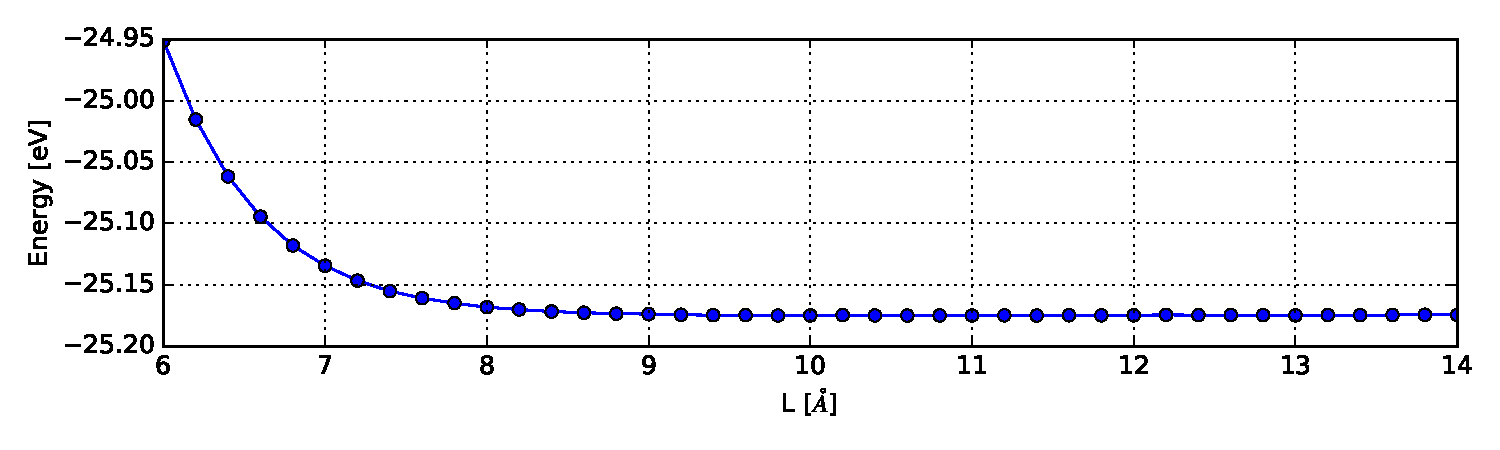
\includegraphics[width = 13cm]{Images/polyacetylene/convergence/unit_cell_width}
	\caption{Ground state energy of relaxed polyacetylene in respect to the width of the unit cell (not in direction of periodic boundary condition).}
	\label{image_poly_width_energy}
\end{figure}
\newpage


\section{Physical Quantities of Polyacetylene}
First, the bond length $a$ in direction of the periodic boundary is calculated (see \cref{image_trans_polyacetylene,image_scheme_dimer}). This quantity corresponds with the half unit cell length (in the direction of periodic boundaries) and thus is calculated by minimizing the ground state energy in respect to the cell length (see \cref{image_poly_cell_len}). Through a quadratic fit the parameter $a = \unit[1.23]{\AA}$ is obtained, that matches the literature value of $\unit[1.2]{\AA}$ (from \cite{PhysRevLett.42.1698}).\\
\begin{figure}[!h]
	\centering
	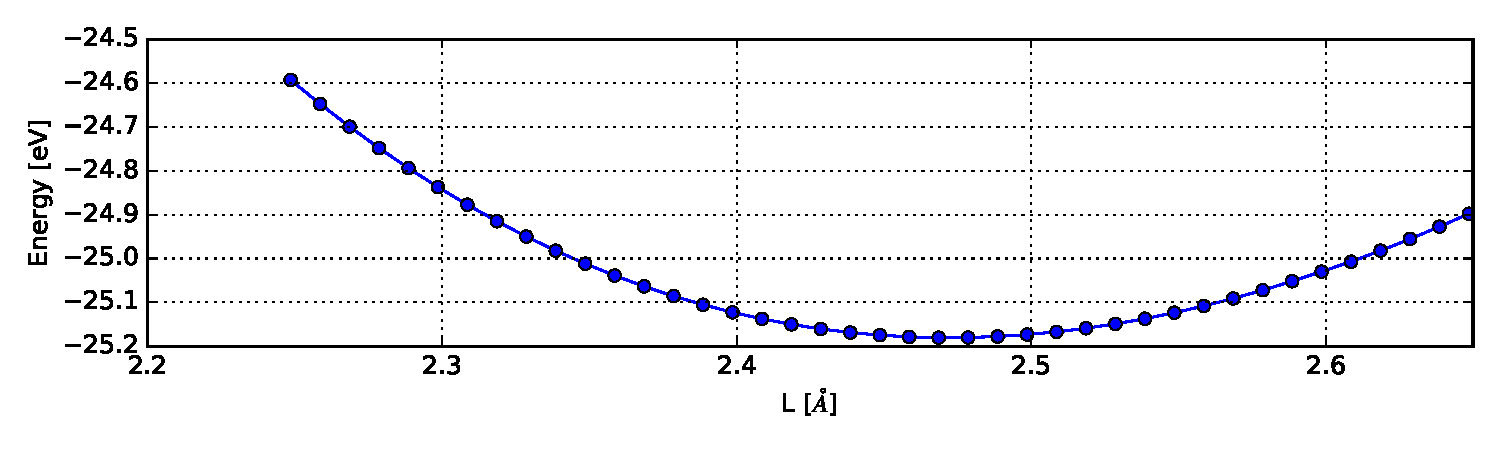
\includegraphics[width = 13cm]{Images/polyacetylene/convergence/unit_cell_length}
	\caption{Ground state energy of relaxed polyacetylene in respect to the length of the unit cell in direction of periodic boundaries.}
	\label{image_poly_cell_len}
\end{figure}
\\
Second, the displacement $u$ of the carbon atoms is checked. Here, no distortion is obtained  at all ($u < \unit[10^{-4}]{\AA}$) by using automatic $k$-point sampling, which doesn't include a $k$-point directly at the edge of the \textsc{Brillouin} zone. If the $k$-points are chosen manually in the way that a $k$-point at the edge of the \textsc{Brillouin} zone is included, a displacement of approximately $u = \unit[5\cdot10^{-3}]{\AA}$ is obtained (see \cref{image_k_point_sampling_assymetry}). In comparison to the literature value of $u = \unit[0.042]{\AA}$ (from \cite{PhysRevLett.42.1698, doi:10.1021/cr990357p}) it is still one order of magnitude too small, but it is known that PBE delocalizes electrons too much, which results in too small distortions and therefore in too small band gaps  \cite{JIANG2009120,PhysRevB.84}.\\
\begin{figure}
	\centering
	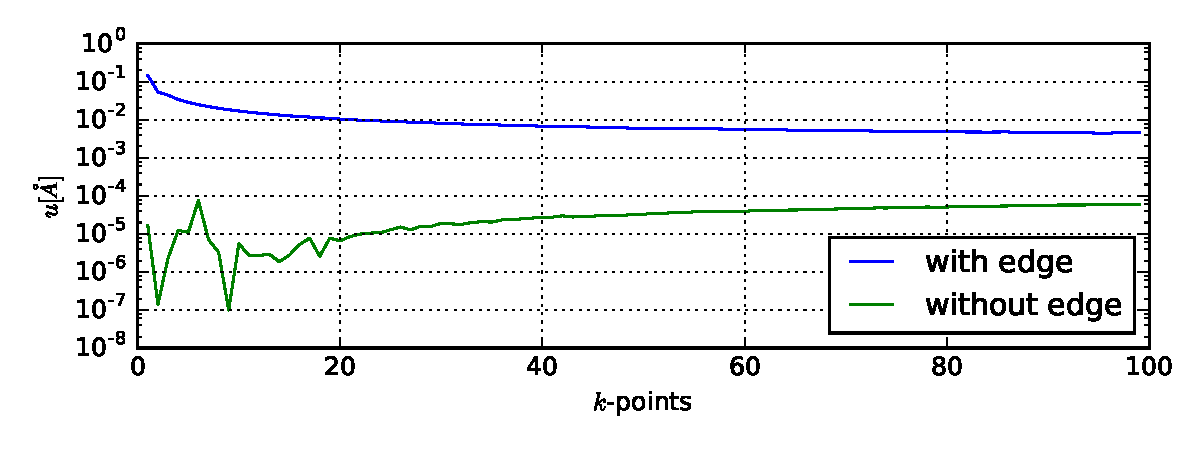
\includegraphics[width = 13cm]{Images/polyacetylene/convergence/polyacetylene_displacement}
	\caption{Displacement $u$ of the carbon atoms in respect to the number of $k$-points for automatic sampling (without $k$-point at the edge of the \textsc{Brillouin} zone) and manually placed $k$-points (with one $k$-point at the edge of the \textsc{Brillouin} zone).}
	\label{image_k_point_sampling_assymetry}
\end{figure}
In \cref{image_potential_with_asymmetry,image_potential_without_asymmetry} the ground state energies in respect to the asymmetry $\nicefrac{u}{u_0}$, whereat $u_0$ denotes the earlier obtained displacement of  $\unit[5\cdot10^{-3}]{\AA}$, can be seen. For the case of $k$-points including the edge of the \textsc{Brillouin} zone (\cref{image_potential_with_asymmetry}), a twofold degeneracy of the ground state corresponding with the displacements $u = \pm u_0$ can be seen, which arises from the symmetry of the problem. In contradiction to this a non degenerate ground state corresponding with no asymmetry is obtained in the case of excluding the edge of the \textsc{Brillouin} zone (\cref{image_potential_without_asymmetry}).\\
\begin{figure}
	\centering
	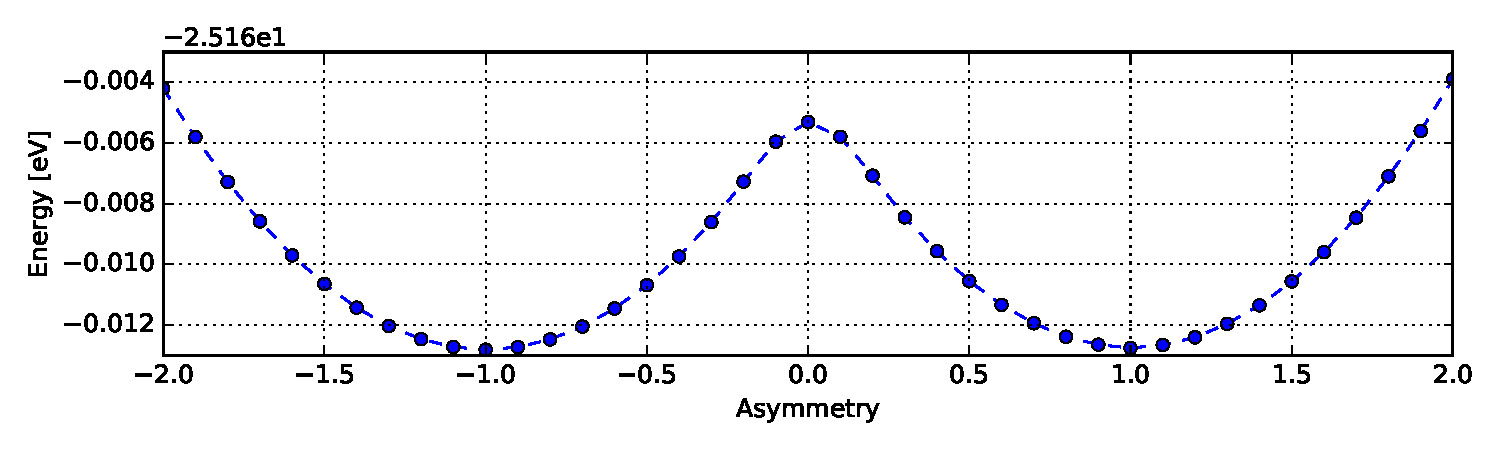
\includegraphics[width = 13cm]{Images/polyacetylene/convergence/Potential_with_asymmetry}
	\caption{Ground state energy for manually displaced CH-groups of polyacetylene for calculations including a $k$-point at the edge of the \textsc{Brillouin} zone.}
	\label{image_potential_with_asymmetry}
\end{figure}
\begin{figure}[!p]
	\centering
	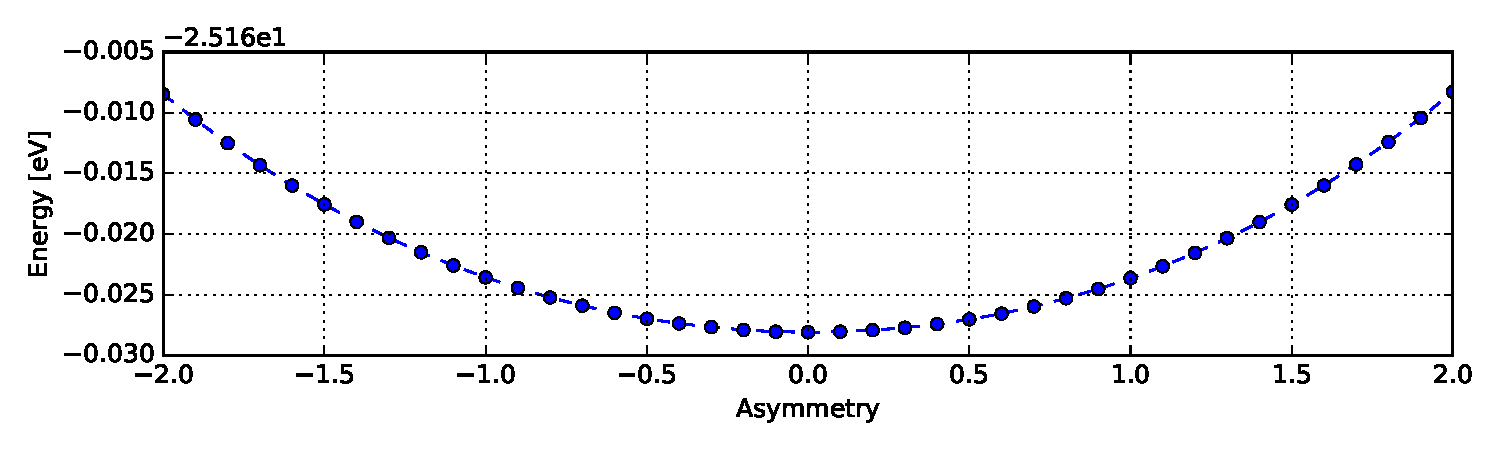
\includegraphics[width = 13cm]{Images/polyacetylene/convergence/Potential_without_asymmetry}
	\caption{Ground state energy for manually displaced CH-groups of polyacetylene for calculations excluding a $k$-point at the edge of the \textsc{Brillouin} zone.}
	\label{image_potential_without_asymmetry}
\end{figure}
\begin{figure}[!p]
	\centering
	\begin{tikzpicture}[show background rectangle, scale = 1]
	\foreach \x in {0,...,7}{
		\draw[line width=2pt] (\x,0) .. controls (\x + 1, 2) and (\x - 1 , 2) .. cycle .. controls (\x + 1, -2) and (\x - 1 , -2) .. cycle;
	}
	\foreach \x in {0, 4}
	\foreach \y in {0, 1}
	\foreach \z in {-1, 1}
	\node at (\x + \y - \z + 1, \z) {\large +};
	\foreach \x in {0, 4}{
		\foreach \y in {0, 1}{
			\foreach \z in {-1, 1}{
				\node at (\x + \y - \z + 1, -\z) {\large -};
	}}}
	\draw[line width = 0.2] (-0.1, -1.8) -- +(-0.3, 0) -- +(-0.3 ,3.6) -- +(0,3.6);
	\draw[line width = 0.2] (1.1, -1.8) -- +(0.3, 0) -- +(0.3 ,3.6) -- +(0,3.6);
	\draw[line width = 0.2] (3.9, -1.8) -- +(-0.3, 0) -- +(-0.3 ,3.6) -- +(0,3.6);
	\draw[line width = 0.2] (7.1, -1.8) -- +(0.3, 0) -- +(0.3 ,3.6) -- +(0,3.6);
	\draw[dotted, line width = 1.5] (-0.6,0) -- (-1,0);
	\draw[dotted, line width = 1.5] (7.6,0) -- (8,0);
	\end{tikzpicture}
	\caption{Scheme: Sign of p-orbitals in a linear chain, that form an alternating $\pi$-bond. The phase difference of two adjacent unit cells, which contain two carbon atoms, is given by $\pi$, whereas the phase difference of two adjacent unit cells, each with four carbon cores, is given by zero.}
	\label{image_scheme_pi_bonds}
\end{figure}
\begin{figure}[!p]
	\centering
	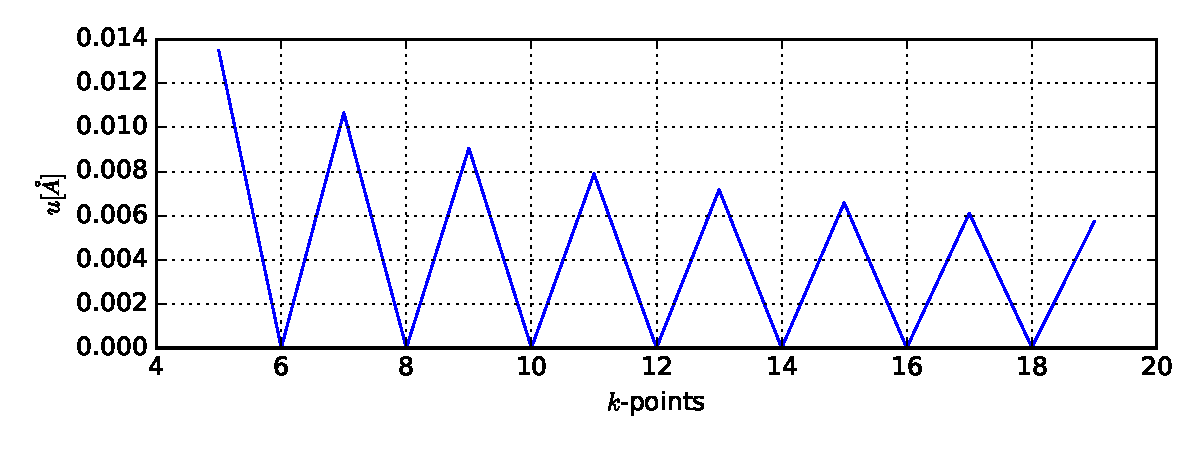
\includegraphics[width = 13cm]{Images/polyacetylene/convergence/displacement_double_cell_poly}
	\caption{Displacement $u$ of the carbon atoms in respect to the number of $k$-points for automatic sampling. The $\Gamma$-point is automatically included for odd numbers of $k$-points, which leads to some asymmetry.}
	\label{image_disp_double_cell_poly}
\end{figure}
\newpage The importance of the $k$-point at the edge of the \textsc{Brillouin} zone can be understood by looking at the sign of the p-orbitals of the carbon atoms, which form an alternating $\pi$-bond (see \cref{image_scheme_pi_bonds}). 
\begin{figure}[!b]
	\centering
	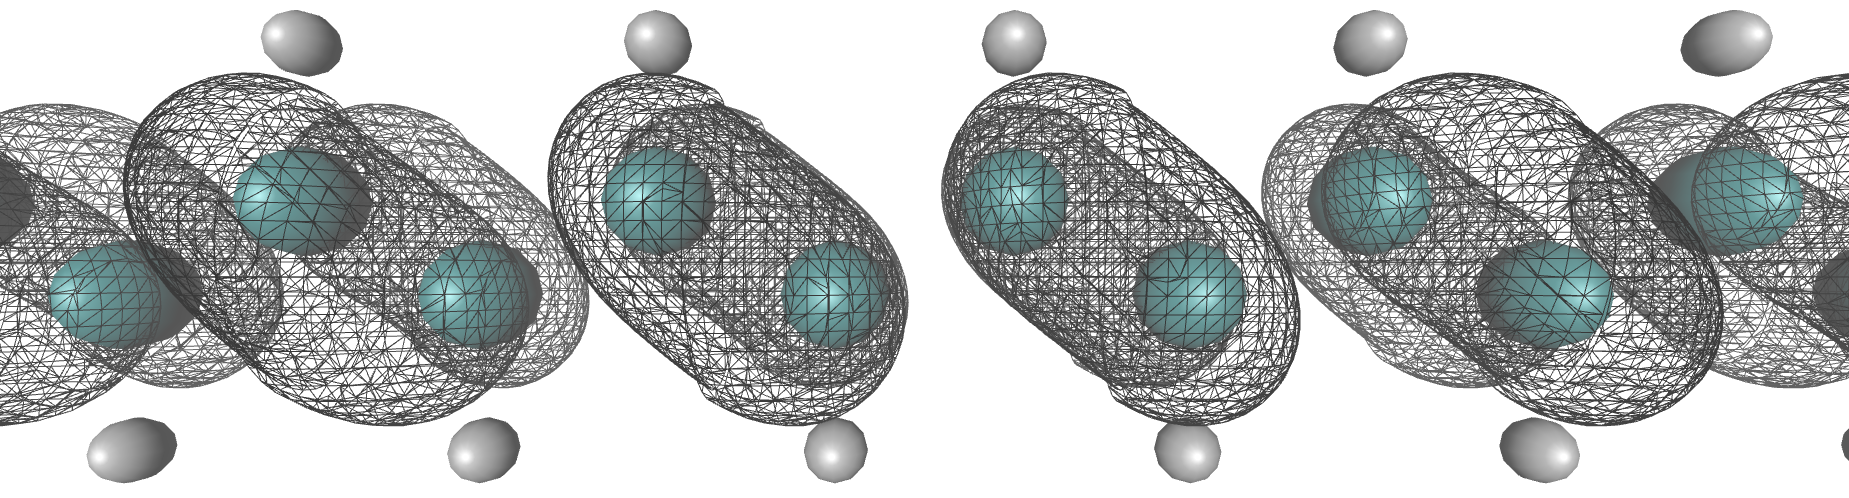
\includegraphics[width = 10cm]{Images/polyacetylene/wavefunctions/Homo}
	\caption{Isosurface for the HOMO-band state at the edge of the \textsc{Brillouin} zone.}
	\label{image_homo1}
\end{figure}
\begin{figure}[!b]
	\centering
	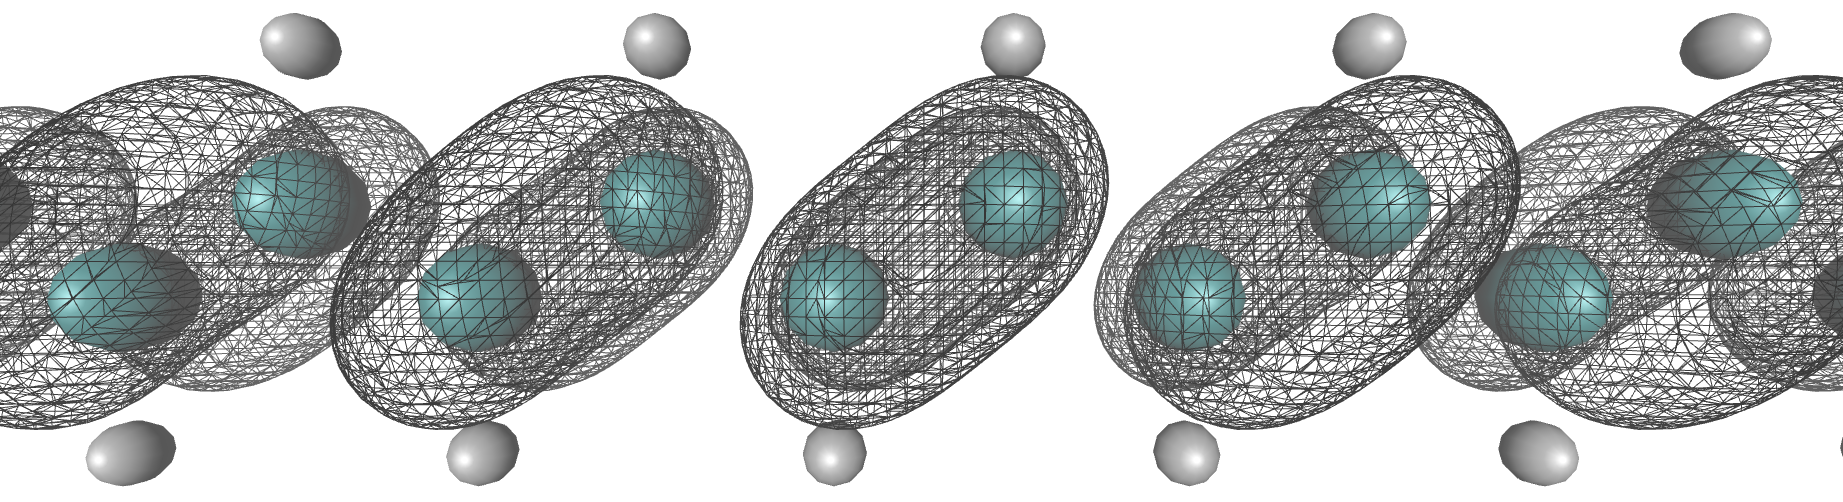
\includegraphics[width = 10cm]{Images/polyacetylene/wavefunctions/LUMO}
	\caption{Isosurface for the LUMO-band state at the edge of the \textsc{Brillouin} zone.}
	\label{image_lumo1}
\end{figure}
\begin{figure}[!b]
	\centering
	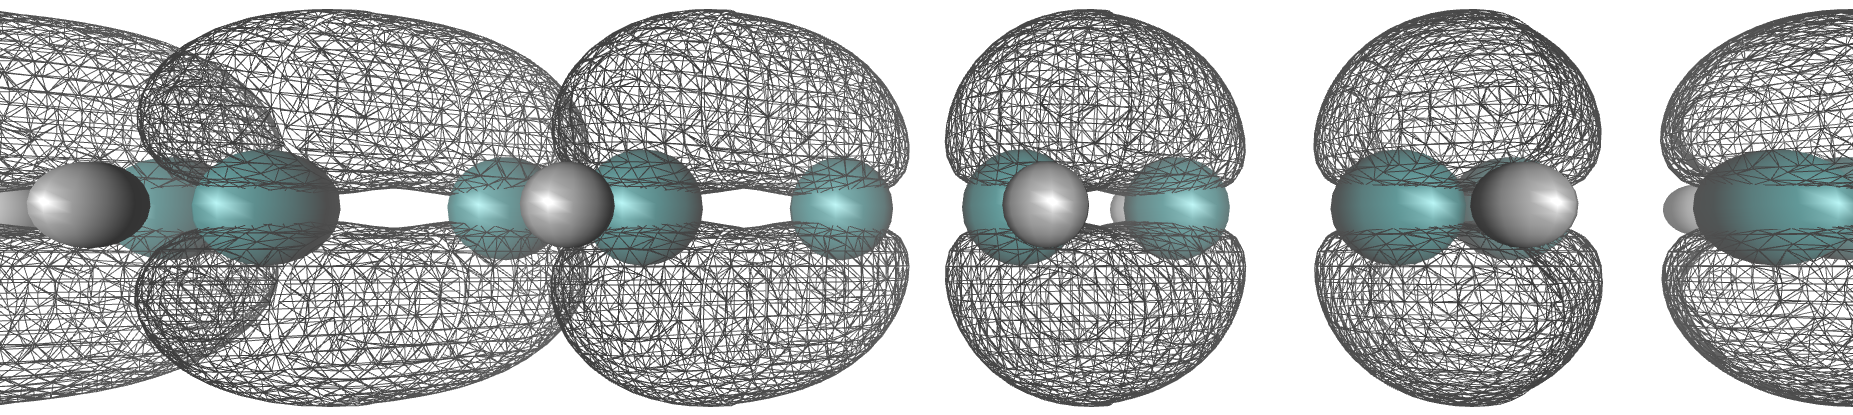
\includegraphics[width = 10cm]{Images/polyacetylene/wavefunctions/HOMO_Side_View}
	\caption{Side view of the isosurface for the HOMO-band state at the edge of the \textsc{Brillouin} zone. The typical 'out of plane' character of the $\pi$-bonds can be seen.}
	\label{image_homo1_side_view}
\end{figure}
Here, a unit cell containing two carbon atoms has a phase shift of $\pi$ between adjacent unit cells, which corresponds with a $k$-point at the edge of the \textsc{Brillouin} zone.\\
Consequently, the $\Gamma$-point is expected to be important for getting an asymmetry in an unit cell containing four carbon atoms, since the phase difference of two such adjacent unit cells has to be $0$ to form alternating $\pi$-bonds. This is checked by simply using automatic $k$-point sampling, which includes the $\Gamma$-point for an odd number of $k$-points automatically. As expected, an alternating behavior for the displacement in respect to the number of $k$-points can be seen in \cref{image_disp_double_cell_poly}.\\
Also, the wave functions of the HOMO- and LUMO-band at the edge of the \textsc{Brillouin} zone show the expected forms (see \cref{image_homo1,image_lumo1,image_homo1_side_view}, where the turquoise balls represent the carbon atoms, the white ones the hydrogen atoms. All plots of isosurfaces are made with VMD \cite{HUMP96}). In particular this means, that the HOMO- and LUMO-band states at the edge of the \textsc{Brillouin} zone have basically the same form but form alternating $\pi$-bonds between opposite pairs of carbon. This would correspond with changing the sign of the p-orbitals of every second carbon atom in \cref{image_scheme_pi_bonds}, which can also be seen directly from the earlier derived eigenstates (see \cref{equation_conduction_eigenstate,equation_valence_eigenstate}). From the symmetry it can be concluded, that for $u=0$ this two states should have the same energy and therefore no band gap is expected.\\
\begin{figure}
	\centering
	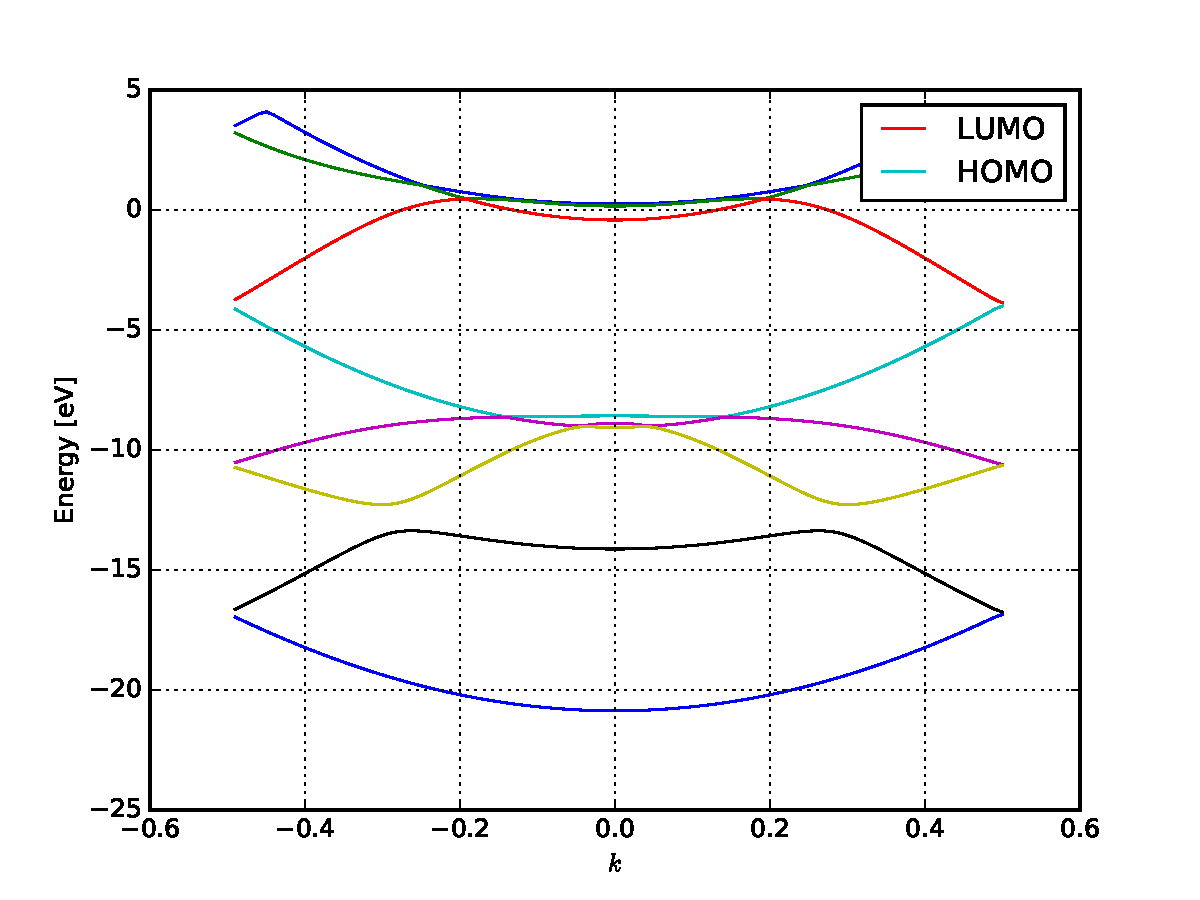
\includegraphics[width = 11cm]{Images/polyacetylene/bands/band_structure}
	\caption{Band structure of relaxed polyacetylene containing the five highest occupied bands and three unoccupied bands.}
	\label{image_band_structure_relaxed_polyacetylene}
\end{figure}
The band structure of the relaxed polyacetylene can be seen in \cref{image_band_structure_relaxed_polyacetylene}. Here and in the following plots of band structures, the $k$-values are given in respect to the basis of the reciprocal lattice and thus a value of $k = \pm 0.5$ corresponds with a state at the edge at the \textsc{Brillouin} zone. As expected a very small band gap of approximately $E_\text{Gap} \approx \unit[0.137]{eV}$ between the HOMO- and LUMO-band can be seen. Again this mismatches the literature value of $E_\text{Gap} = \unit[1.4]{eV}$  (from \cite{PhysRevLett.42.1698}) by a complete order of magnitude. The form of the HOMO- and LUMO-band in the outer regions seems to be in good accordance with the predicted form (compare \cref{equation_energy_band}):
\begin{align}
E_k &= \pm \sqrt{\left(2t_0\cos(ka)\right)^2+\left(2\delta\sin(ka)\right)^2}
\label{equation_explicit_energy_band}
\end{align} 
\begin{figure}[!p]
	\centering
	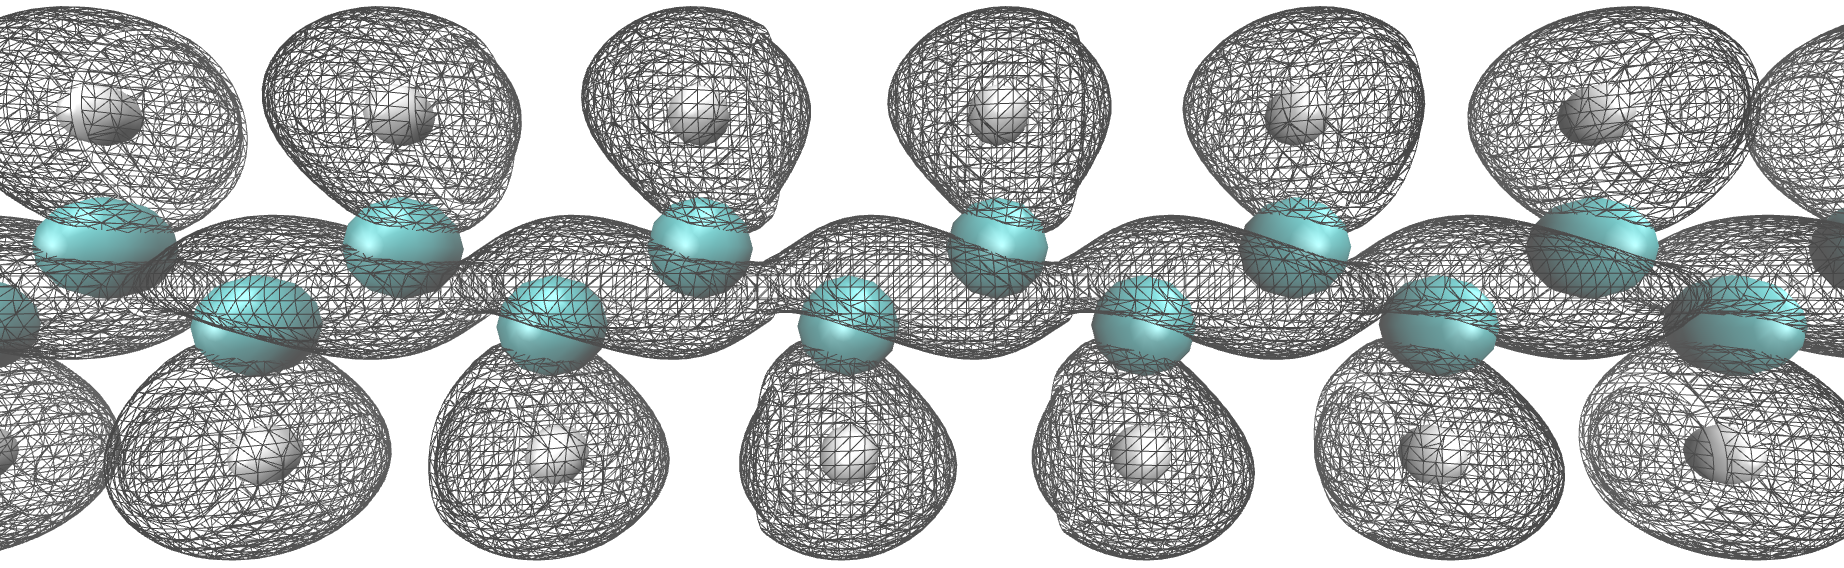
\includegraphics[width = 12cm]{Images/polyacetylene/wavefunctions/Homo_mid_k}
	\caption{Isosurface for the HOMO-band state at the $\Gamma$-point.}
	\label{image_homo_mid_k}
\end{figure}
\begin{figure}[!p]
	\centering
	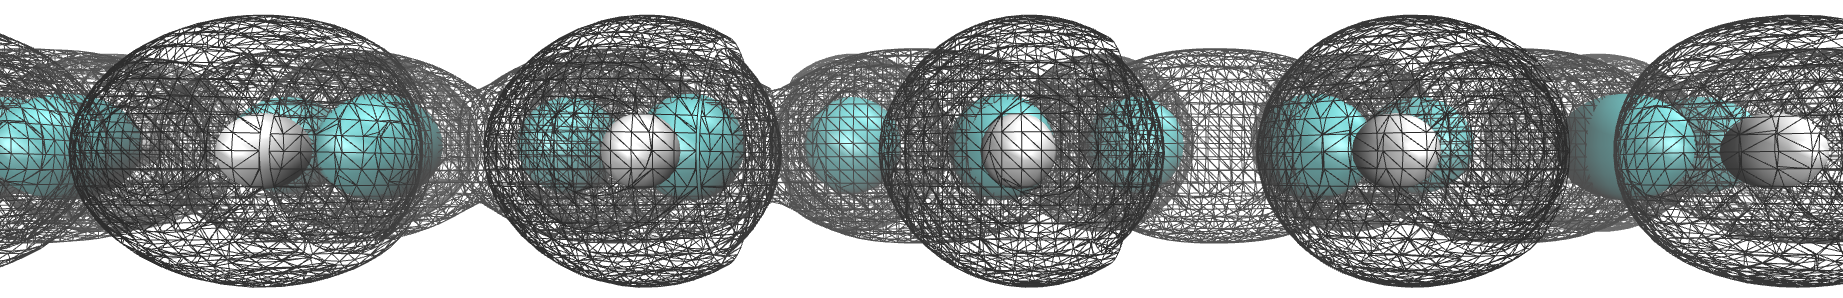
\includegraphics[width = 12cm]{Images/polyacetylene/wavefunctions/Homo_mid_k_Side_View}
	\caption{Side view of the isosurface for the HOMO-band state at the $\Gamma$-point without an 'out of plane' character.}
	\label{image_homo_mid_k_side_view}
\end{figure}
\begin{figure}[!p]
	\centering
	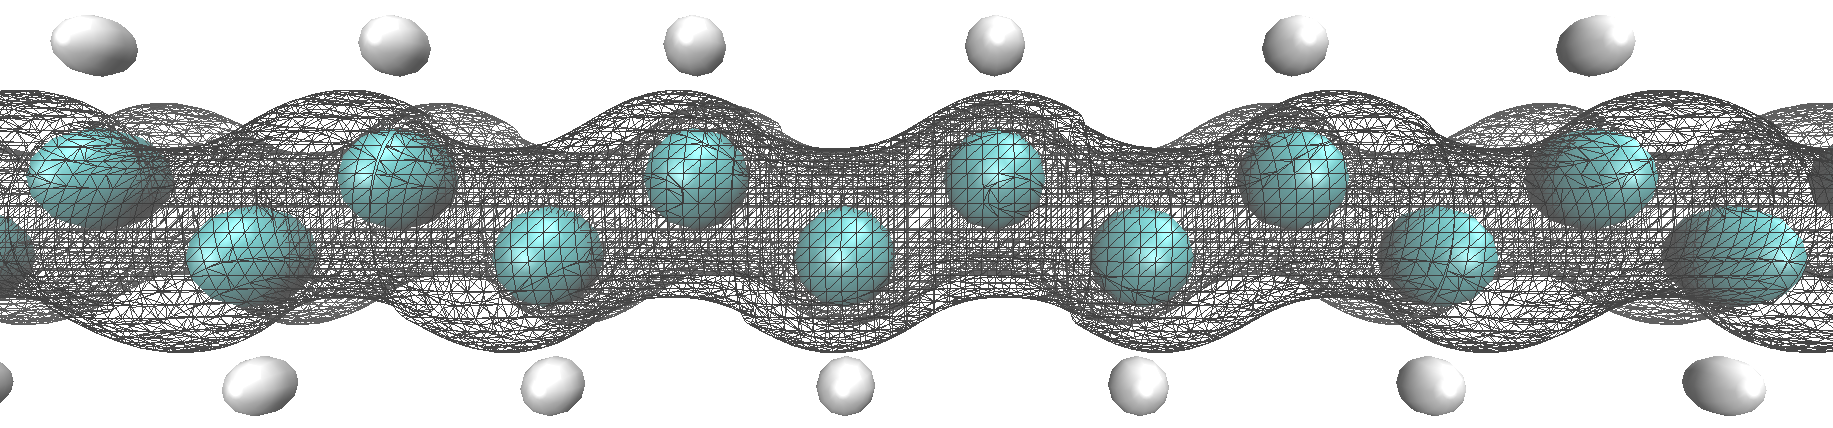
\includegraphics[width = 12cm]{Images/polyacetylene/wavefunctions/Mid_band_2}
	\caption{Isosurface of the third band at the $\Gamma$-point.}
	\label{image_third_band}
\end{figure}
\begin{figure}[!p]
	\centering
	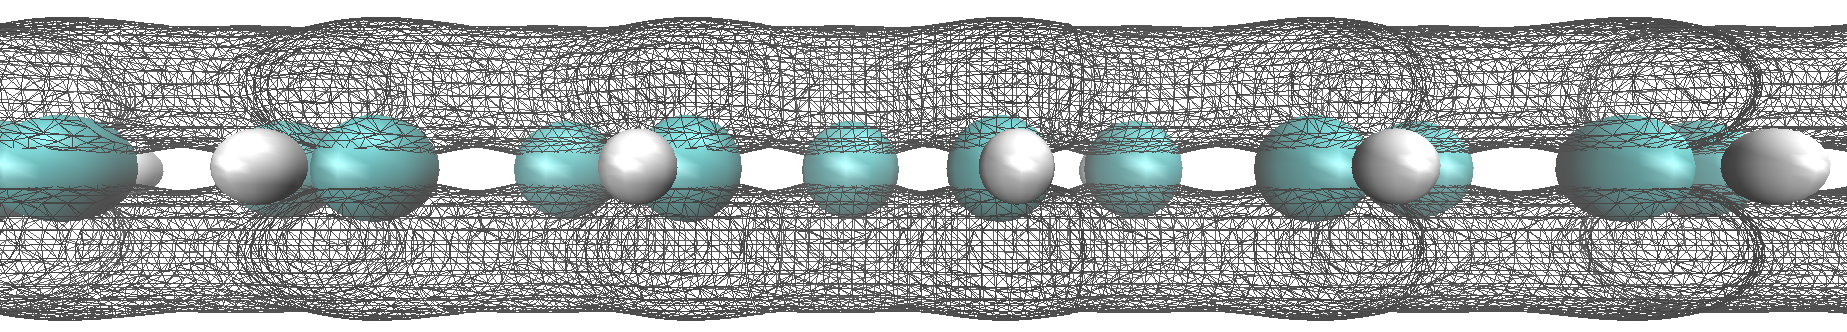
\includegraphics[width = 12cm]{Images/polyacetylene/wavefunctions/Mid_band_2_Side_View}
	\caption{Side view of the third band at the $\Gamma$-point, showing an 'out of plane' character.}
	\label{image_third_band_side_view}
\end{figure}
In the central region some interaction between the bands occurs, which leads to the well known effect of \emph{avoided crossings} \cite{ashcroft}. \newpage This effect can also be seen by looking at the wave functions of the third and the HOMO-band at the $\Gamma$-point (see \cref{image_homo_mid_k,image_homo_mid_k_side_view,image_third_band,image_third_band_side_view}), which shows that for the $\Gamma$-point the third band and not the HOMO-band corresponds with the p-orbitals. Further it can be seen that the state of the third band at the $\Gamma$-point drawn in the schematic way of \cref{image_scheme_pi_bonds} would have the same sign for all p-orbitals in the upper row and the other sign for all states in the lower row (see \cref{image_scheme_p_orbitals_gamma_point}).\\
\begin{figure}
	\centering
	\begin{tikzpicture}[show background rectangle, scale = 1]
	\foreach \x in {0,...,7}{
		\draw[line width=1pt] (\x,0) .. controls (\x + 1, 2) and (\x - 1 , 2) .. cycle .. controls (\x + 1, -2) and (\x - 1 , -2) .. cycle;
	}
	\foreach \x in {0,...,7}{
		\foreach \y/\s in {-1/+, 1/-}{
			\node at (\x, \y) {\large \s};}}
	\draw[dotted, line width = 1.5] (-0.6,0) -- (-1,0);
	\draw[dotted, line width = 1.5] (7.6,0) -- (8,0);
	\end{tikzpicture}
	\caption{Scheme: Sign of p-orbitals of the state for the HOMO-band at the $\Gamma$-point.}
	\label{image_scheme_p_orbitals_gamma_point}
\end{figure}
To get the hopping parameter $t_0$ a fit with the form of \cref{equation_explicit_energy_band} is done to a continuous combination of the third, forth and fifth band (see \cref{image_band_fit_t0}), because band interactions aren't handled in this simple model\footnote{From the context can be seen if an offset is used for the fits. In most of the cases a fixed offset at the middle of the band gap is used.}. Thus a hopping parameter of $\unit[2.62]{eV}$ is obtained, which matches the literature value of $\unit[2.5]{eV}$ very well (from \cite{PhysRevLett.42.1698}).\\
To calculate the phonon coupling constant the following relation is used:
\begin{align}
	\alpha &= \frac{1}{8} \frac{\partial E_\text{Gap}}{\partial u}
\end{align}
Thus the band gap is calculated for different displacements $u$ and a linear fit is applied to this data (see \cref{image_alpha_fit}), whereat the phonon coupling constant is calculated from the slope. In this way a value of $\alpha = \unitfrac[3.95]{eV}{\AA}$ is obtained, which again matches very well a literature value of $\alpha = \unitfrac[4.1]{eV}{\AA}$.\\
Finally the band gap for a manually displacement in accordance to the literature value of $u = \unit[0.042]{\AA}$ (from \cite{PhysRevLett.42.1698, doi:10.1021/cr990357p}) is calculated (see \cref{image_manually_displaced_poly_bandstructure}). This yields a band gap of $E = \unit[1.27]{eV}$, which is quite good in comparison with the literature value of $E_\text{Gap} = \unit[1.4]{eV}$ (see \cite{PhysRevLett.42.1698}).\\
A short summary of the results is given in \cref{table_summary_polyacetylene}.\\
\begin{figure}
	\centering
	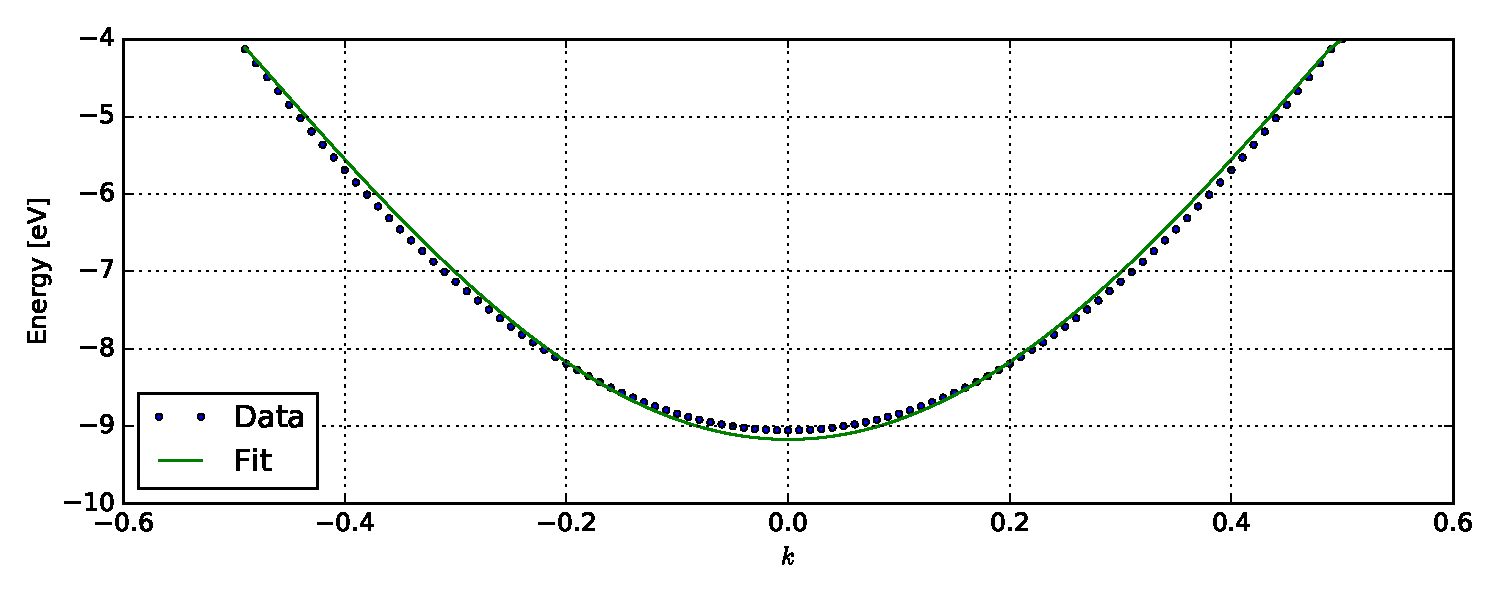
\includegraphics[width = 13cm]{Images/polyacetylene/bands/band_fit}
	\caption{Fit of the derived band form to a continuous combination of the third, forth and fifth band from polyacetylene.}
	\label{image_band_fit_t0}
\end{figure}
\begin{figure}
	\centering
	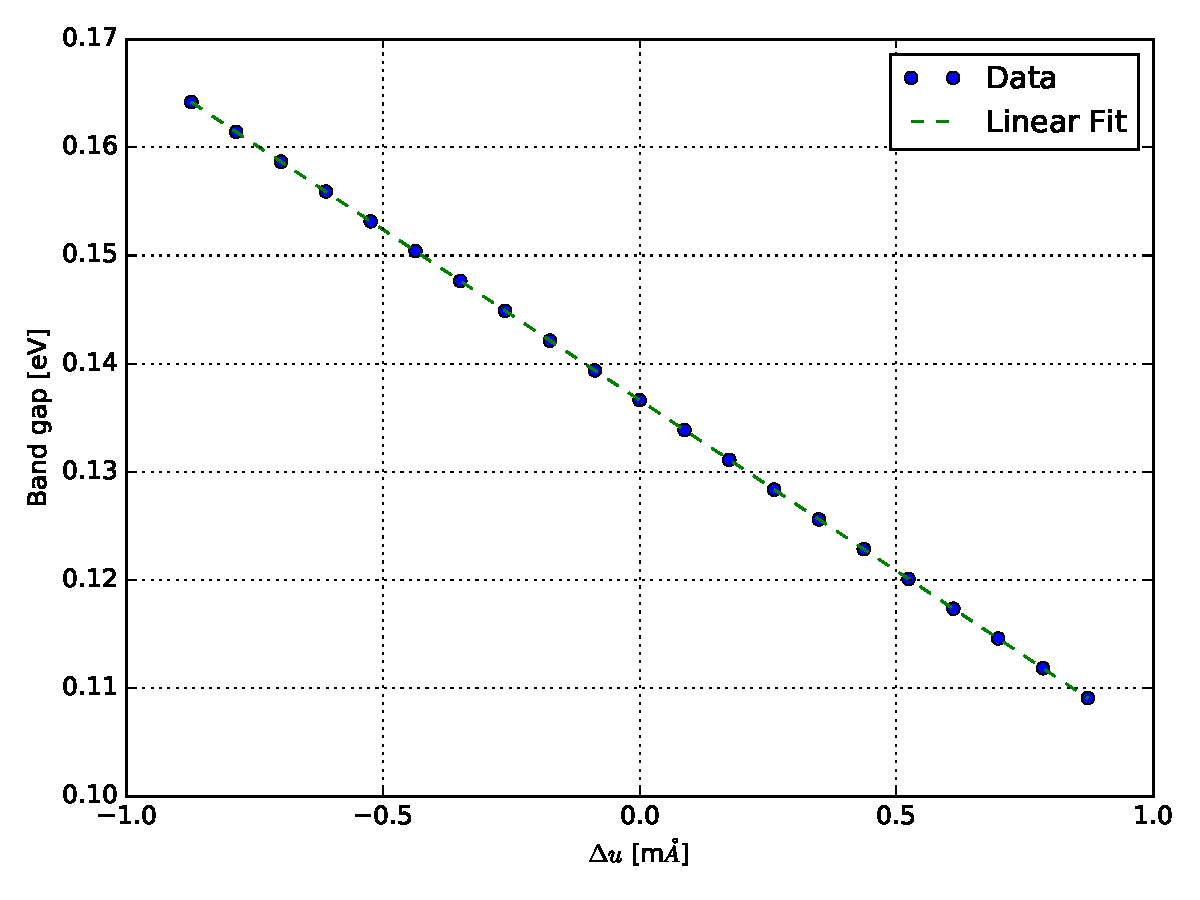
\includegraphics[width = 13cm]{Images/polyacetylene/bands/alpha}
	\caption{Band gap for manually displacements $u$ with a linear fit.}
	\label{image_alpha_fit}
\end{figure}
\begin{figure}
	\centering
	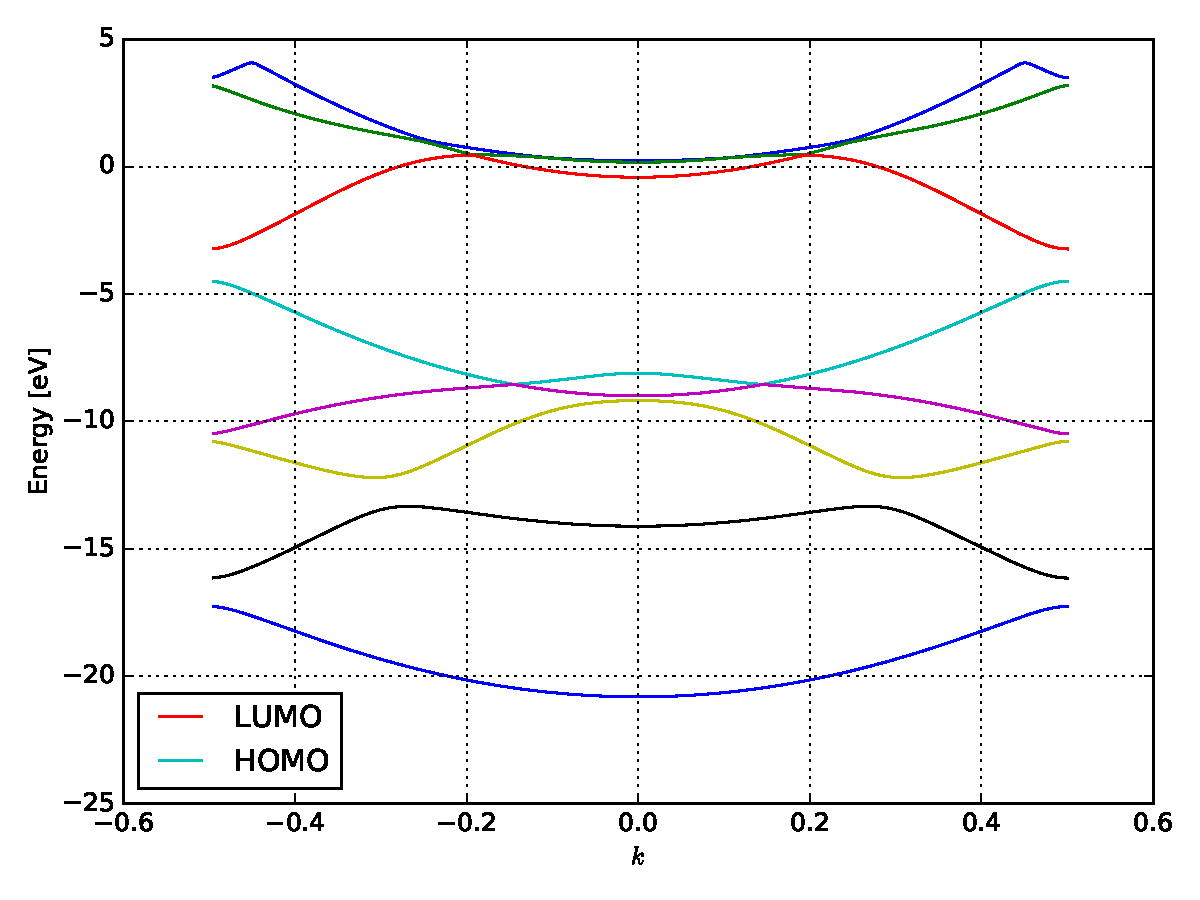
\includegraphics[width = 11cm]{Images/polyacetylene/bands/bandstructure_manually_displaced}
	\caption{Band structure of manually displaced polyacetylene.}
	\label{image_manually_displaced_poly_bandstructure}
\end{figure}
\begin{table}[]
	\centering
	\begin{tabular}{l|c|c}
	Quantety & Calculated Value & Literature Value (\cite{PhysRevLett.42.1698, doi:10.1021/cr990357p})\\
	\hline \hline
	&&\\[-.3cm]
	Bond length \hfill$a [\unit{\AA}]$ & $1.23$ & $1.2$\\ \hline&&\\[-.3cm]
	Displacement \hfill$u [\unit{\AA}]$& $0 - 5\cdot10^{-3}$ & $0.042$\\ \hline&&\\[-.3cm]
	Band gap (manually displaced)\hfill$E_\text{Gap} [\unit{eV}]$ & $0.137\quad(1.27)$ & $1.4$\\ \hline &&\\[-.3cm]
	Hopping parameter \hfill$t_0 [\unit{eV}]$ & $2.62$ & $2.5$ \\ \hline&&\\[-.3cm]
	Phonon coupling constant \hspace*{2cm}$\alpha [\unitfrac{eV}{\AA}]$& $3.95$ & $4.1$
	\end{tabular}
	\caption{Summary of the results for polyacetylene.}
	\label{table_summary_polyacetylene}
\end{table}


\section{Constraint Density Functional Theory}
\label{section_constraint_density_functonal_theory}
In this section the influences of charging different regions by using cDFT is studied and two alternative methods for calculating the hopping parameter $t_0$ are tested. First, this is done for a system as simple as possible, namely a chain of equidistant hydrogen atoms. But before doing this, some technical issues with cDFT are discussed.
\subsection{Technical Details}
\label{section_technical_issues}
\begin{figure}
	\centering
	\begin{subfigure}{0.45\textwidth}
		\centering
		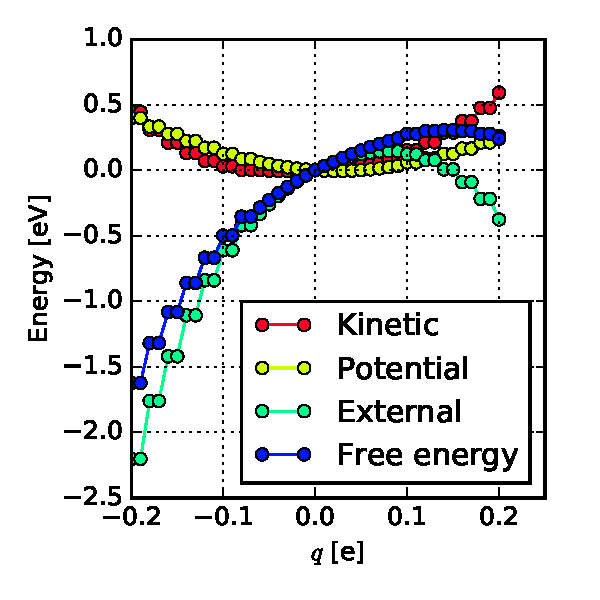
\includegraphics[width = \textwidth]{Images/Hydrogen/charging/energy_contributions_asymmetric}
		\caption{Initial}
		\label{image_contributions_initial}
	\end{subfigure}\hspace*{1cm}
	\begin{subfigure}{0.45\textwidth}
		\centering
		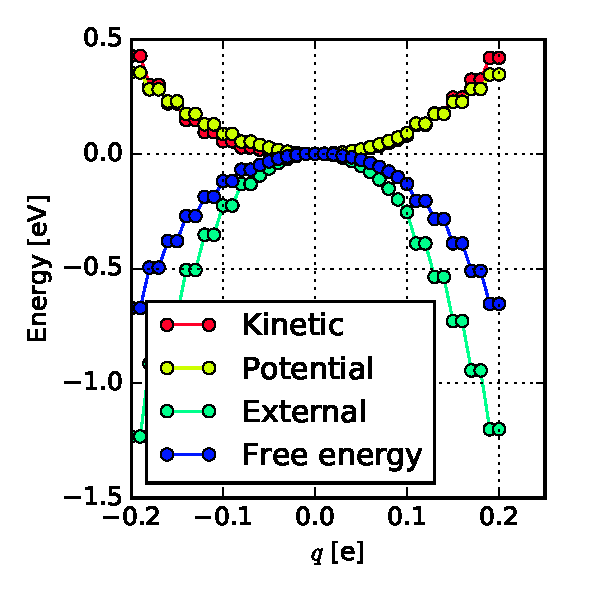
\includegraphics[width = \textwidth]{Images/Hydrogen/charging/energy_contributions_symmetric}
		\caption{Corrected}
		\label{image_contributions_corrected}
	\end{subfigure}
	\caption{Different energy contributions for the hydrogen chain in respect to the displaced charge. The offsets are set to zero for $q=0$.}
\end{figure}
\begin{figure}
	\centering
	\begin{subfigure}{0.45\textwidth}
		\centering
		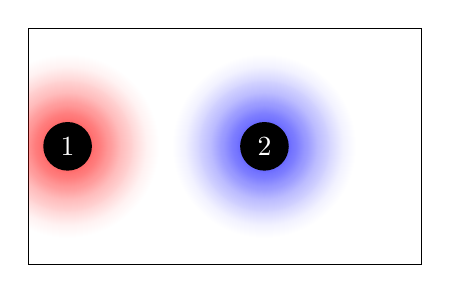
\begin{tikzpicture}[]
		\begin{scope}
		\clip [draw] (-.5, -1.5) rectangle (4.5, 1.5);
		\foreach \x/\color in {0/red, 2.5/blue}{
			\foreach \r in {0, 0.01, ..., 1}{
				\fill[opacity = \r * 0.03, fill = \color] (\x, 0) circle ({2.5 * (.5 - 0.5 * \r)});}}
		\foreach \x/\num in {0/1, 2.5/2}{
			\node[fill = black, shape = circle, text = white] at (\x, 0)	 {\num};}
		\end{scope}
		\end{tikzpicture}
		\caption{\textsc{Gaussian} curves cut at periodic boundary.\\}
	\end{subfigure}\hspace*{1cm}
	\begin{subfigure}{0.45\textwidth}
		\centering
		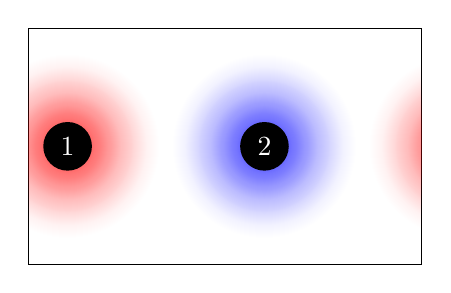
\begin{tikzpicture}
		\begin{scope}
		\clip [draw] (-.5, -1.5) rectangle (4.5, 1.5);
		\foreach \x/\color in {0/red, 2.5/blue, 5/red}{
			\foreach \r in {0, 0.01, ..., 1}{
				\fill[opacity = \r * 0.03, fill = \color] (\x, 0) circle ({2.5 * (.5 - 0.5 * \r)});}}
		\foreach \x/\num in {0/1, 2.5/2}{
			\node[fill = black, shape = circle, text = white] at (\x, 0)	 {\num};}
		\end{scope}
		\end{tikzpicture}
		\caption{\textsc{Gaussian} curves continued at opposite site for periodic boundary.}
	\end{subfigure}
	\caption[Schemes: \textsc{Gaussian} curves from cDFT with periodic boundary conditions.]{Schemes: \textsc{Gaussian} curves for two regions (\textcolor{red}{red} and \textcolor{blue}{blue}) used as weights for the integration/summation over the electron density to calculate the charge in each region.}
	\label{image_periodicity_gaussians}
\end{figure} 
By using cDFT with periodic boundary conditions, different asymmetric contributions to the ground state energy can be seen (see \cref{image_contributions_initial}), which isn't expected due to the symmetry of the problem. Therefore, it shouldn't matter if charge is moved from region one to region two or the other way around. And indeed, this issue is caused by some shortcoming in the cDFT source code, namely the cut of the \textsc{Gaussian} curves at periodic boundaries (see \cref{image_periodicity_gaussians}). Correcting this resolved the issues with the asymmetry (see \cref{image_contributions_corrected}).\\
Next, an issue with the quantity $q$ is discussed:\\
From the tight-binding point of view, $q$ denotes the charge belonging to some distinct core. On the other hand, there is the $q$ appearing in the cDFT code, describing the integral over the charge density weighted with some \textsc{Gaussian} curves centered at the core positions. Even if they look somehow similar, they can't be simply assumed to be the same. To get some relation between them a 'tight-binding' $q$ has to be calculated out of the charge density. Here the most natural approach seems to associate the charge at any point with the nearest core. This can be done by dividing the unit cell into two separate parts and integrating the charge density over each of this regions (see \cref{image_tight_binding_q_regions}).\\
For a test system of an infinite hydrogen chain (see \cref{section_hydrogen_chain}), a linear dependency between the tight-binding and cDFT charge can be seen in \cref{image_qs_hydrogen}. The proportionality constants derived from the fits depend on the value for $\sigma$ of the \textsc{Gaussian} curves from cDFT. For $\sigma = \unit[0.24]{\AA}$ the relation $q_\text{tb} \approx 1.10\cdot q_\text{cDFT}$ and for $\sigma = \unit[0.32]{\AA}$ the relation $q_\text{tb} \approx 1.17\cdot q_\text{cDFT}$ is obtained.\\
\begin{figure}
	\centering
	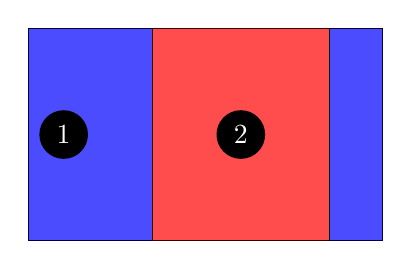
\begin{tikzpicture}[scale = .9]
	\begin{scope}
	\clip [draw] (-.5, -1.5) rectangle (4.5, 1.5);
	\draw [fill = blue, opacity = 0.7] (-0.5, -1.5) rectangle (4.5, 1.5);
	\draw [fill = white, opacity = 1] (1.25, -1.5) rectangle (3.75, 1.5);
	\draw [fill = red, opacity = 0.7] (1.25, -1.5) rectangle (3.75, 1.5);
	\foreach \x/\num in {0/1, 2.5/2}{
		\node[fill = black, shape = circle, text = white] at (\x, 0)	 {\num};}
	\end{scope}
	\end{tikzpicture}
	\caption[Scheme: Integration regions to calculate a 'tight-binding' q]{Scheme: Integration regions (\textcolor{red}{red} and \textcolor{blue}{blue}) to calculate a 'tight-binding charge'.}
	\label{image_tight_binding_q_regions}
\end{figure}
\begin{figure}
	\centering
	\begin{subfigure}{0.49\textwidth}
		\centering
		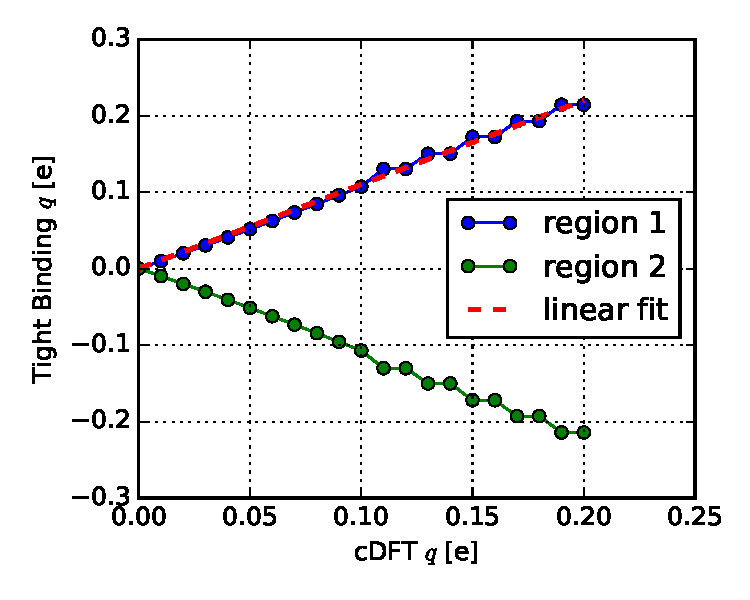
\includegraphics[width = \textwidth]{Images/Hydrogen/charging/qs_normal_sigma}
		\caption{$\sigma = \unit[0.24]{\AA}$}
		\label{}
	\end{subfigure}\hspace*{.5cm}
	\begin{subfigure}{0.49\textwidth}
		\centering
		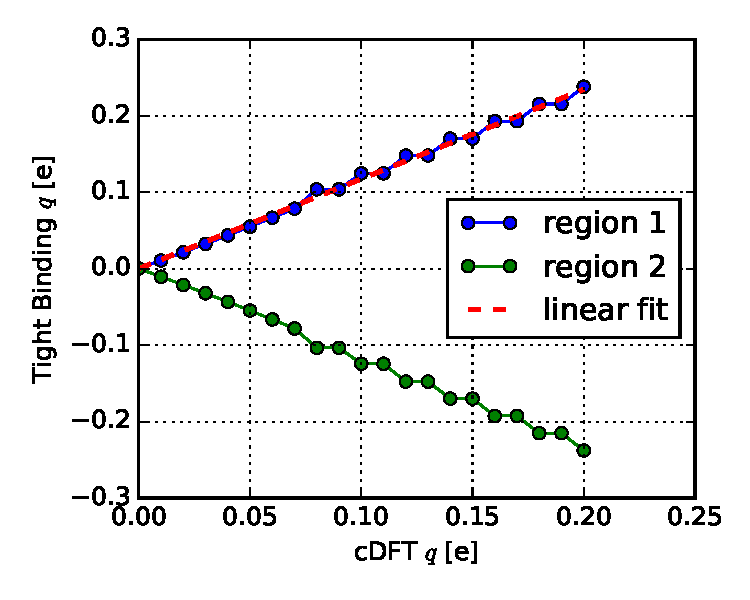
\includegraphics[width = \textwidth]{Images/Hydrogen/charging/qs_other_sigma}
		\caption{$\sigma = \unit[0.32]{\AA}$}
		\label{}
	\end{subfigure}
	\caption{Tight binding $q$ in respect to the cDFT q with a linear fit for different $\sigma$.}
	\label{image_qs_hydrogen}
\end{figure}
Finally, the relevance of choosing appropriate initial cDFT potential heights $U_i$ is shown.\\ For no displaced charge $q = 0$ the external potentials should vanish ($U_i = 0$), since this corresponds with the natural state. As can be seen in \cref{image_potential_asymmetrys}, this is not the case if symmetric initial potential heights $U_1 = U_2 > 0$ are used for a test system of an infinite hydrogen chain (see \cref{section_hydrogen_chain}). This effect can be understood by looking at the amount of charge in the second region (free) for different charges (determined with cDFT) in the first region (see \cref{image_charge_correlation}). Here a perfect anticorrelation (correlation value of $-1$) is obtained, which means that for any charge pushed out of region one some proportional charge ($\approx 86\%$) gets pushed into region two. Consequently a symmetric increase/decrease of $U_1$ and $U_2$ has a smaller effect on the amount of charge in the two regions.  Thus, the initial potentials are always chosen to be antisymmetric. This is of even bigger relevance for bigger systems like polyacetylene.
\begin{figure}
\centering
\begin{minipage}{0.49\textwidth}
\centering
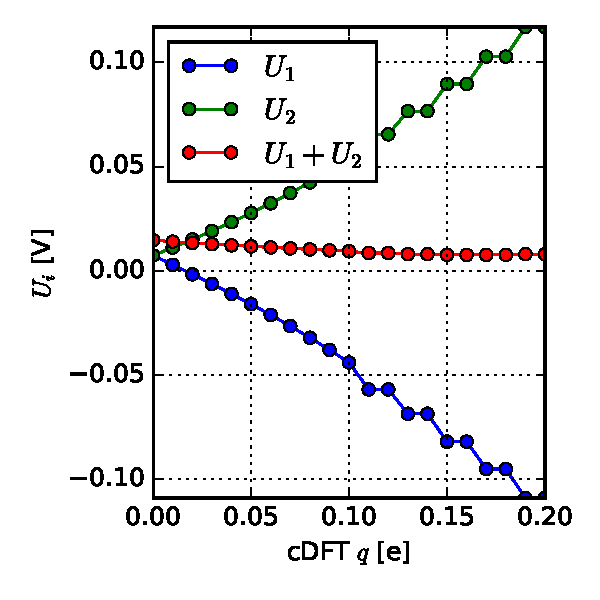
\includegraphics[width = \textwidth]{Images/Hydrogen/charging/Potential_asymmetry}
\caption{cDFT potentials $U_i$ and their sum in respect to the displaced charge for symmetric initial potentials \mbox{($U_1 = U_2 > 0$)}.}
\label{image_potential_asymmetrys}
\end{minipage}\hspace*{.5cm}
\begin{minipage}{0.49\textwidth}
\centering
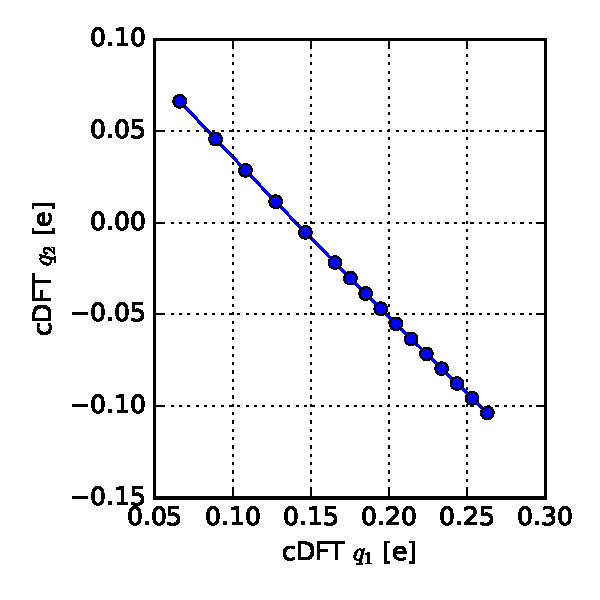
\includegraphics[width = \textwidth]{Images/Hydrogen/charging/charge_correlation}
\caption{Charge in the second region (not chosen) in respect to the charge in the first region (chosen).\\}
\label{image_charge_correlation}
\end{minipage}
\end{figure}

\subsection{Chain of Hydrogen Atoms}
\label{section_hydrogen_chain}
Even if there's no distortion, a unit cell with two hydrogen atoms is needed, because later the application of the external potentials and the consequential charge displacement will break the symmetry. First, the unit cell length for the lowest ground state energy is determined to $L = \unit[2.0]{\AA}$ (see \cref{image_hydrogen_unit_cell_length}).
\begin{figure}[]
	\centering
	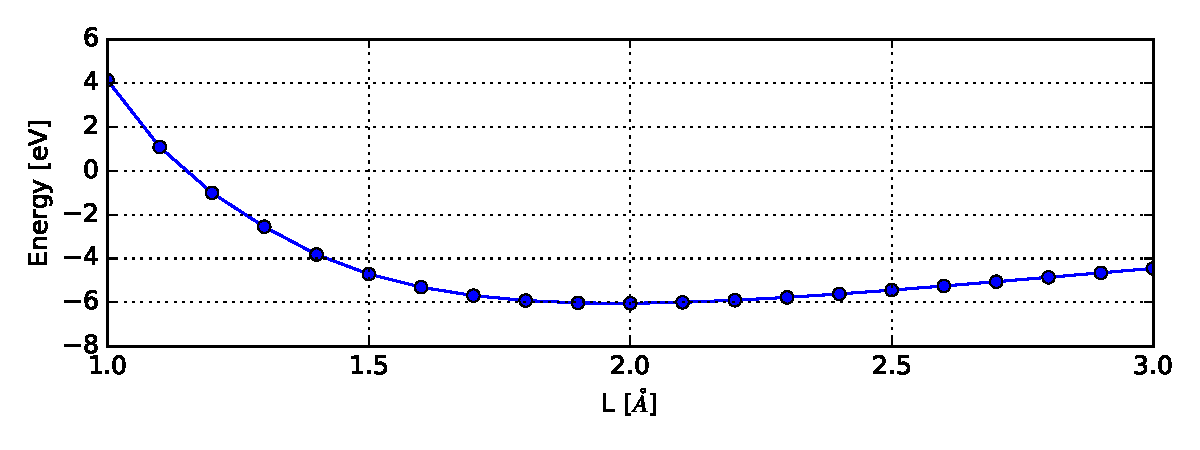
\includegraphics[width = 12cm]{Images/Hydrogen/convergence/hydrogen_length}
	\caption{Ground state energy of a unit cell containing two equidistant hydrogen atoms in respect to the unit cell length in direction of the periodic boundaries.}
	\label{image_hydrogen_unit_cell_length}
\end{figure}
\begin{figure}[]
	\centering
	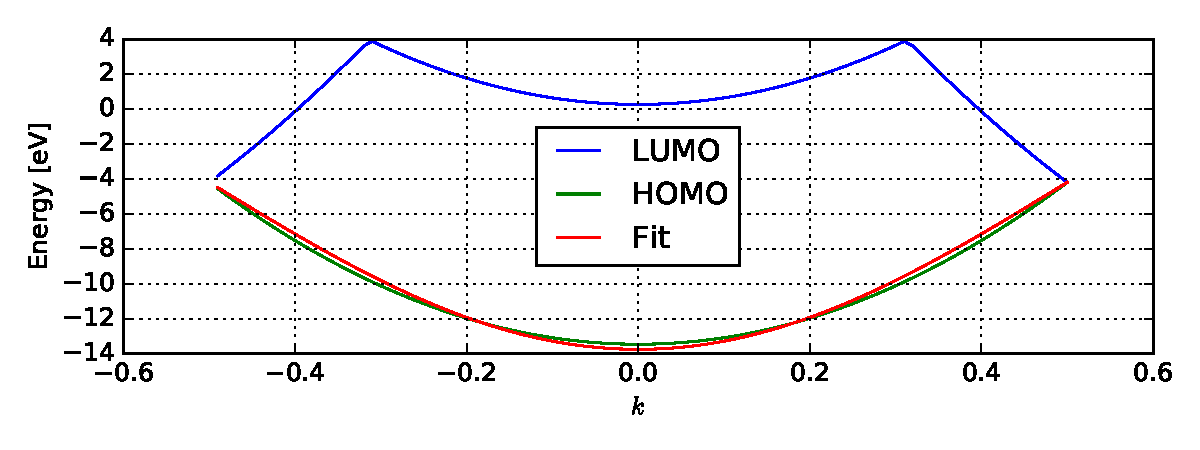
\includegraphics[width = 12cm]{Images/Hydrogen/bands/hydrogen_band_structure}
	\caption{Band structure of a hydrogen chain with a fit to its HOMO-band.}
	\label{image_hydrogen_band_structure}
\end{figure}
\\
As can be seen in \cref{image_hydrogen_band_structure}, the HOMO-band is in good accordance with the expected form\footnote{Since there's no distortion $\Delta_k = 0$ (compare \cref{equation_energy_band}).} of:
\begin{align}
	E_k = -2t_0\cos(ka)
\end{align}
from which the hopping parameter $t_0 = \unit[4.8]{eV}$ is obtained. This value is used as reference later.\\
In the next step, an appropriate modification of the tight-binding model is needed to describe the charge displacements due to cDFT. The simplest approach would be, that the charge displacement does not change the Hamiltonian $\mathcal{H}_k$ and the wave functions $\Psi_k{(v)}$ change in the following way:
\begin{align}
\Psi_k^{(v)}(q_\text{tb}) &= \sqrt{\frac{1}{2}-\frac{q_\text{tb}}{2}}c_k^{\dagger(e)}- \sqrt{\frac{1}{2}+\frac{q_\text{tb}}{2}}\frac{\epsilon_k - i \Delta_k}{|E_k|}c_{k}^{\dagger(o)}
\end{align}
where $q_\text{tb}$ denotes the displaced tight-binding charge. These states show the needed behaviour:
\begin{align}
	2\sum_k\left\langle\Psi_k^{(v)}(q_\text{tb})\Big|\hat{n}_k^{(e/o)}\Big|\Psi_k^{(v)}(q_\text{tb})\right\rangle &= N \left(1 \pm q_\text{tb}\right)
\end{align}
which corresponds with a charge transfer of $q_\text{tb}$ in each unit cell. Further, these states have an energy expectation value of:
\begin{align}
\left\langle\Psi_k^{(v)}(q_\text{tb})\Big|\mathcal{H}_{k}\Big|\Psi_k^{(v)}(q_\text{tb})\right\rangle &= -\sqrt{1-q^2_\text{tb}} |E_k|
\label{equation_method_1_energies}
\end{align}
Finally, the assumption that the ground state energy can be approximated by the sum of the single electron energies is made, which leads to the expression:
\begin{align}
E_0(q_\text{tb}) &= -\frac{4Nt_0}{\pi} \sqrt{1-q^2_\text{tb}}
\label{equation_ground_state_energy_charge}
\end{align}
Using the proportionality constants $c$ between $q_\text{tb}$ and $q_\text{cDFT}$ (see \cref{section_technical_issues}), the ground state energy can be fitted to the following expression\footnote{$N=2$, because the unit cell contains two hydrogen atoms.} (compare \cref{equation_ground_state_energy_charge}):
\begin{align}
	E_0(q_\text{cDFT}) &= -\frac{8t_0}{\pi} \sqrt{1 - \left(c\cdot q_\text{cDFT}\right)^2}
\end{align}
Next an appropriate value for the standard deviation $\sigma$ of the \textsc{Gaussian} curves has to be determined. A too small $\sigma$ would localize the electrons too much and thus make the displacement of charge more difficult. On the contrary, a too big $\sigma$ would lead to more displaced charge than needed and consequently make the charge transfer also more difficult. In consequence, there should be a value of $\sigma$, for which the displacement of charge becomes the easiest. Out of the previous considerations this $\sigma$ is expected to give a good match of the \textsc{Gaussian} curves with the electron density. As can be seen in \cref{image_gaussian_sigmas_hydrogen}, this is the case for $\sigma \approx \unit[0.24]{\AA}$ (smallest curvature). Consequently, this $\sigma$ is used for the following calculations if not otherwise mentioned.\\
\begin{figure}[!t]
	\centering
	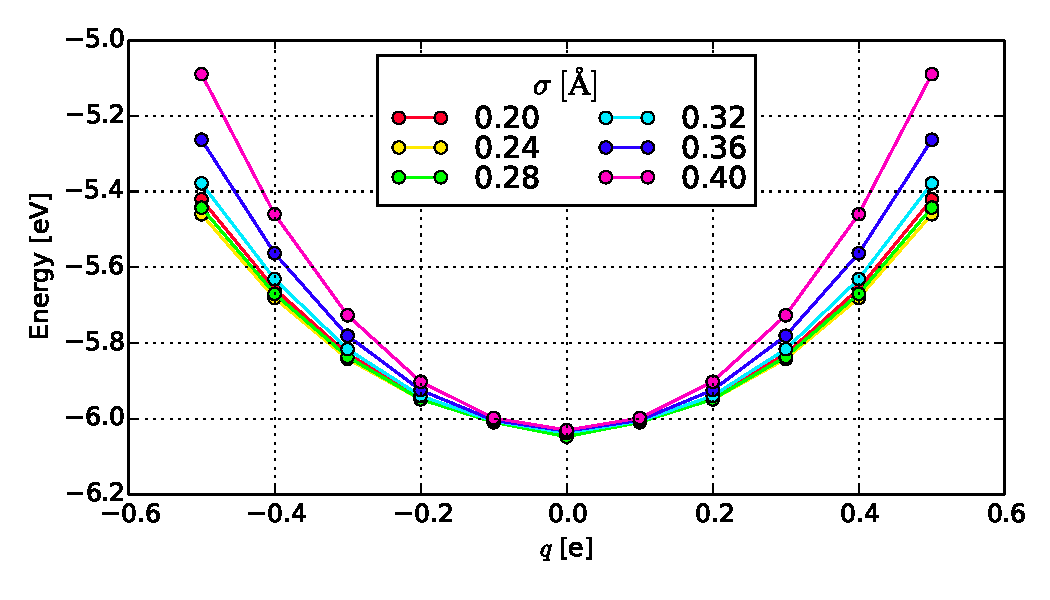
\includegraphics[width = 9.5cm]{Images/Hydrogen/charging/gaussian_sigmas}
	\caption{Ground state energy of the hydrogen chain in respect to the displaced charge for different standard deviations $\sigma$ of the \textsc{Gaussian} curves.}
	\label{image_gaussian_sigmas_hydrogen}
\end{figure}
\begin{figure}[]
	\centering
	\begin{subfigure}{0.49\textwidth}
		\centering
		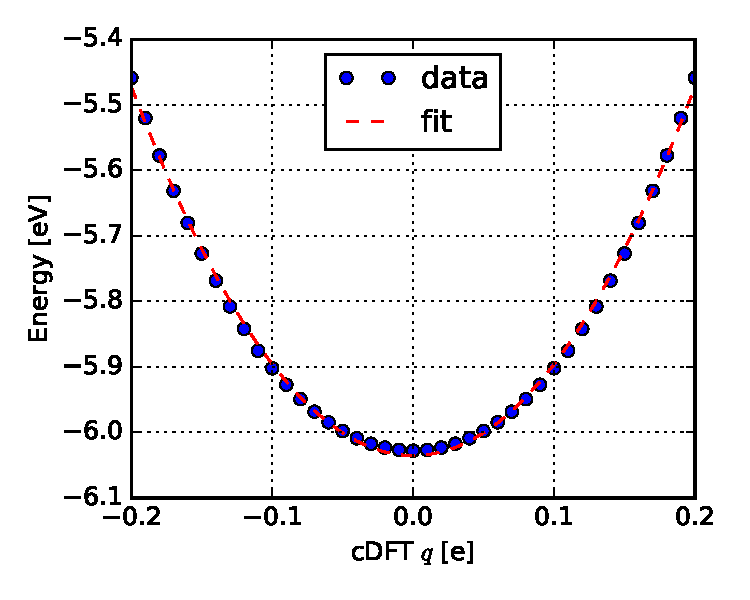
\includegraphics[width = \textwidth]{Images/Hydrogen/charging/energy_fit_normal_sigma}
		\caption{$\sigma = \unit[0.24]{\AA}$}
		\label{}
	\end{subfigure}\hspace*{.5cm}
	\begin{subfigure}{0.49\textwidth}
		\centering
		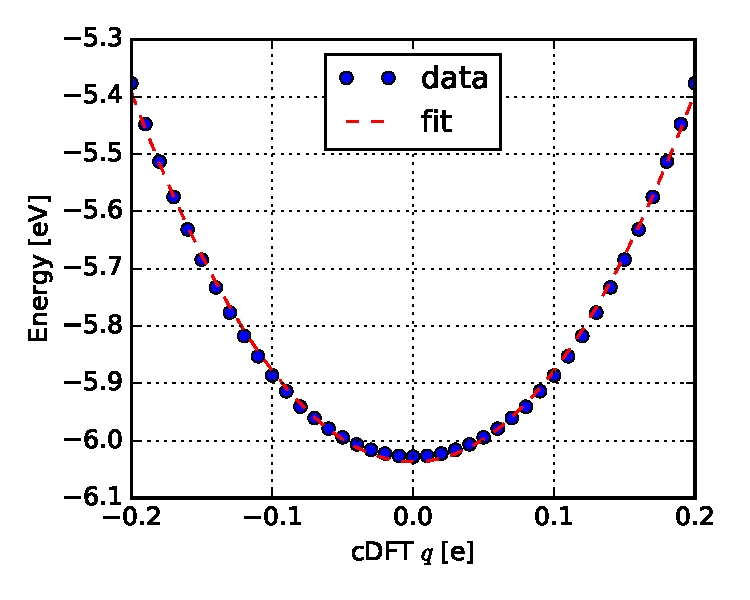
\includegraphics[width = \textwidth]{Images/Hydrogen/charging/energy_fit_other_sigma}
		\caption{$\sigma = \unit[0.32]{\AA}$}
		\label{}
	\end{subfigure}
	\caption{Ground state energy in respect to the displaced charge for different $\sigma$.}
	\label{image_ground_state_hydrogen_qs}
\end{figure}
\newpage
As can be seen in \cref{image_ground_state_hydrogen_qs}, the fits match the data for both $\sigma$ well. The so obtained hopping parameters in respect to different $\sigma$ and corresponding proportionality constants $c$ are:
\begin{table}[!h]
\centering
\begin{tabular}{c|c|c}
$t_0 [\unit{eV}]$ & $\sigma [\unit{\AA}]$ & $c$\\
\hline \hline
9.6&0.18&1.15\\
9.0&0.24&1.10\\
9.0&0.28&1.12\\
9.1&0.32&1.17\\
9.5&0.40&1.36\\
\end{tabular}
\end{table}\\

Two things can be seen from this:\\
First, the hopping parameters do not match the earlier calculated value of $t_0 = \unit[4.8]{eV}$ and thus there must have been some wrong assumptions in the derivation. Second, the values for different $\sigma$ show a tolerable deviation if the correct proportionality constants are used. This would make the choice of an appropriate $\sigma$ much simpler, since the physical quantities would not strongly depend on it.\\
A possible reason why this method yields wrong values could be that the sum of the single particle energies can not be assumed to be equal to the ground state energy. For example the \textsc{Coulomb} energy of the electrons in the field of the other electrons is added twice and terms of the exchange correlation energy are left out. Also the assumption that all $k$-points contribute equally to the charge displacement could be wrong, which can be tested easily. Assuming that the $q_\text{tb} = q(k)$ in \cref{equation_method_1_energies} yields:
\begin{align}
	q(k) &= 1 - \left(\frac{\left\langle\Psi_k^{(v)}(q_\text{tb})\Big|\mathcal{H}_{k}\Big|\Psi_k^{(v)}(q_\text{tb})\right\rangle}{\left|E_k\right|}\right)^{2}
\end{align}
\begin{figure}
	\centering
	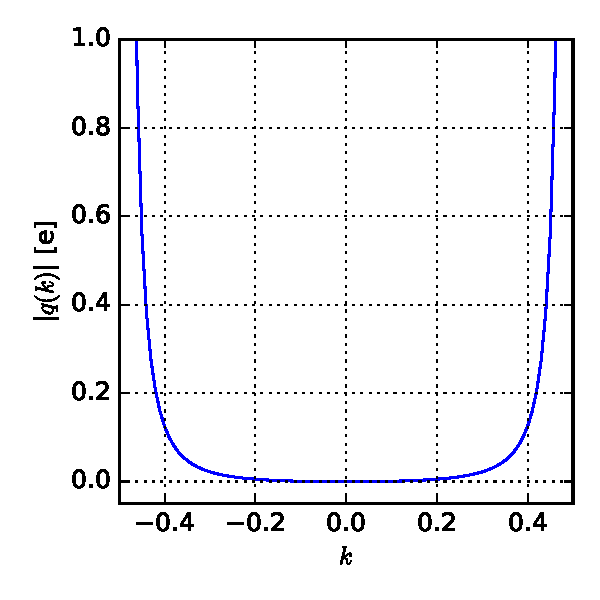
\includegraphics[width = 0.4\textwidth]{Images/Hydrogen/charging/charge_vs_k}
	\caption{Displaced charge in respect to $k$ in a simplified tight binding picture.}
	\label{image_tight_binding_q_vs_k}
\end{figure}
Assuming that the expression $\left\langle\Psi_k^{(v)}(q_\text{tb})\Big|\mathcal{H}_{k}\Big|\Psi_k^{(v)}(q_\text{tb})\right\rangle$ corresponds with the band structure energies from cDFT, the form of $q(k)$ can be seen in \cref{image_tight_binding_q_vs_k}, which is obviously not constant. It can be seen that in this simplified tight-binding picture the states close to the edge of the \textsc{Brillouin} zone contribute most to the charge displacement. Furthermore the $q(k)$ diverges for $k = \pm \nicefrac{1}{2}$, which shows again the exceptional properties of the high symmetry points in the reciprocal space. At least the increase at the edges can be understood intuitively, since the kinetic energy of the electrons contains terms proportional to $k^2$ and thus a bigger contribution to conductivity can be expected. Hence, a modification of the initial tight binding model is searched, that describes the influences on the band structure correctly.\\
The second approach to do this is the following:\\
Modify the hopping Hamiltonian to decrease/increase the energies at the even/odd positions (matrix notation):
\begin{align}
\begin{pmatrix*}[c]
0 & \epsilon_k + i \Delta_k \\
\epsilon_k - i \Delta_k & 0
\end{pmatrix*} 
&\to 
\begin{pmatrix*}[c]
-V & \epsilon_k + i \Delta_k \\
\epsilon_k - i \Delta_k & V
\end{pmatrix*}
\end{align}
with the eigenenergies $E_k = \pm \sqrt{V^2+\epsilon_k^2+\Delta_k^2}$ and the eigenstates\footnote{the valence state corresponds with the lower signs.} (vector notation):
\begin{align}
\vv{\Psi}_k(V) &= \frac{1}{\sqrt{2\left(E_k^2\mp V|E_k|\right)}}\cdot \begin{pmatrix*}[c]
-V\pm \sqrt{V^2+\epsilon_k^2+\Delta_k^2}\\
\epsilon_k - i \Delta_k
\end{pmatrix*}
\end{align}
For $V=0$ this matches the previous result.\\
\begin{figure}
	\centering
	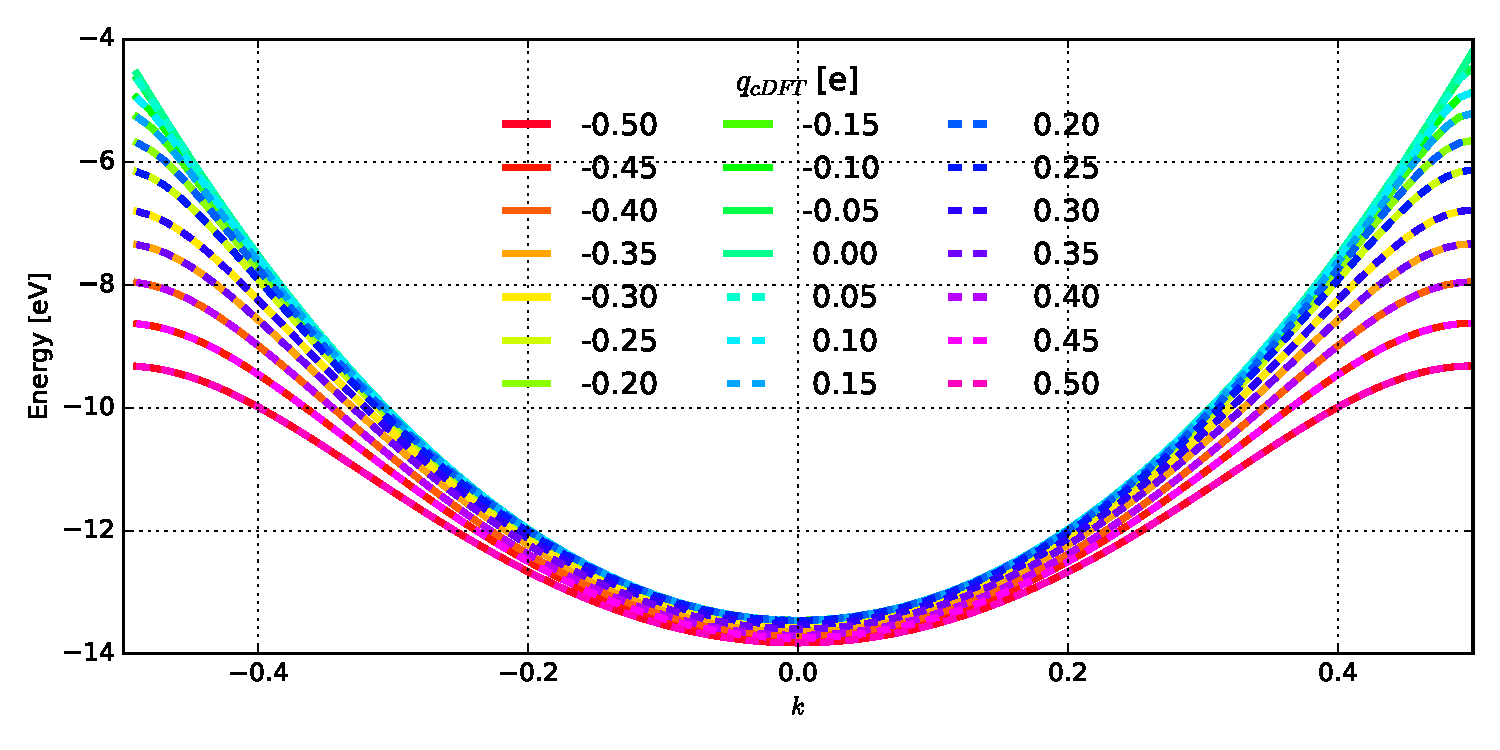
\includegraphics[width = 12cm]{Images/Hydrogen/charging/band_structure_q_1}
	\caption{HOMO- and LUMO-band of the hydrogen chain for different charge displacements.}
	\label{image_hydrogen_charged_bands}
\end{figure}
Next, the band structure for the hydrogen chain with different charge displacements is calculated (see \cref{image_hydrogen_charged_bands}). As expected from the symmetry, the form of the band structures do not depend on the direction (sign) of the charge displacement. It can also be seen, that the influence of charging is bigger for $k$-points closer to the edge of the \textsc{Brillouin} zone and that the HOMO-bands are systematically shifted to lower energies. Both aligns the predictions of the second approach perfectly.
Since there's no distortion in the unit cell, the expected HOMO-band form becomes:
\begin{align}
E_k &= -\sqrt{V^2 + \left(2t_0\cos(ka)\right)^2}
\end{align}
Hence, the energy at the edge of the \textsc{Brillouin} zone is expected to show the following form in respect to the energy $V$ (cosine vanishes):
\begin{align}
E_\text{edge}(V) &= -\left|V\right|
\end{align}
\begin{figure}[!p]
\centering
\begin{minipage}{0.49\textwidth}
\centering
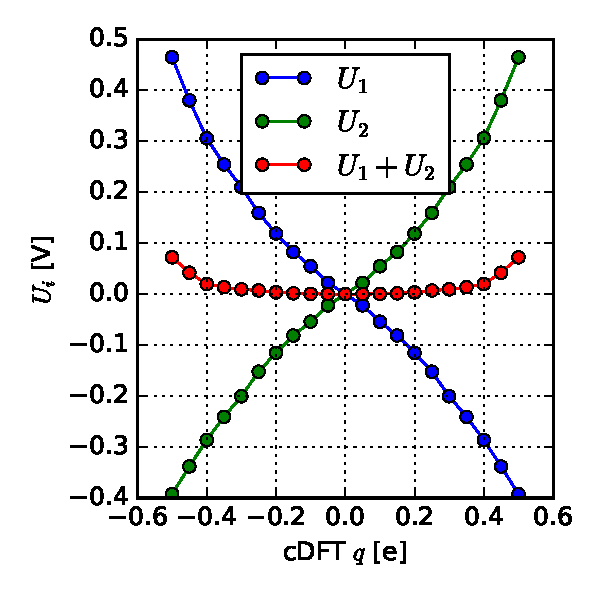
\includegraphics[width = \textwidth]{Images/Hydrogen/charging/potential_q_1}
\caption{cDFT potentials in respect to the displaced charge.\\}
\label{image_potentials_qs_1}	
\end{minipage}\hspace*{.5cm}
\begin{minipage}{0.49\textwidth}
\centering
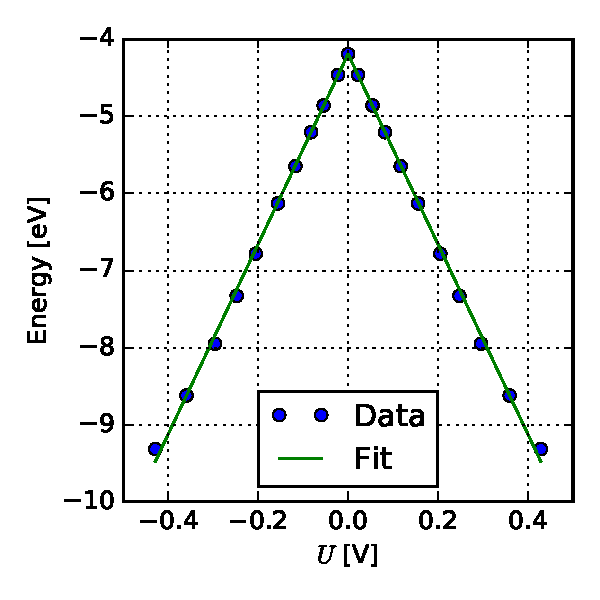
\includegraphics[width = \textwidth]{Images/Hydrogen/charging/border_energy_q_1}
\caption{Band energy for $k = 0.5$ in respect to the external potential with fit.}
\label{image_edge_energy_qs_1}
\end{minipage}
\end{figure}
Here, the heights of the potentials $U_i$ from cDFT correspond with the energy $V$, wherefore a proportionality between them is assumed. Thus, the cDFT potentials should fulfill the condition $U_1 = - U_2$, which is approximately the case (see \cref{image_potentials_qs_1}). Thus, in the following $U = \frac{1}{2}(U_1 - U_2)$ is used as corresponding quantity to $V$.
The proportionality constant between $U$ and $V$ is obtained by fitting
\begin{align}
	E_\text{edge} &= -\left|c \cdot U\right|
\end{align}
to the band energies at the edge of the \textsc{Brillouin} zone (see \cref{image_edge_energy_qs_1}). The fit seems appropriate and yields a value of $c = \unit[12.3]{e}$.\\
This can be used to fit the function
\begin{align}
	E\left(k, U\right) &= - \sqrt{\left(cU\right)^2 + \left(2t_0\cos(ka)\right)^2}
\end{align}
in $t_0$ to the calculated band structures for different charge displacements (see \cref{image_hydrogen_3D_2}). The fit seems to describe the general form very well and yields a hopping parameter of $t_0 = \unit[4.6]{eV}$. This differs slightly from the earlier obtained value of $t_0 = \unit[4.8]{eV}$, but a look on the slices in \cref{image_hydrogen_3D_slices} shows that for no displaced charge $q = 0$ the fit and data still match very nicely.\\
\begin{figure}[!p]
	\centering
	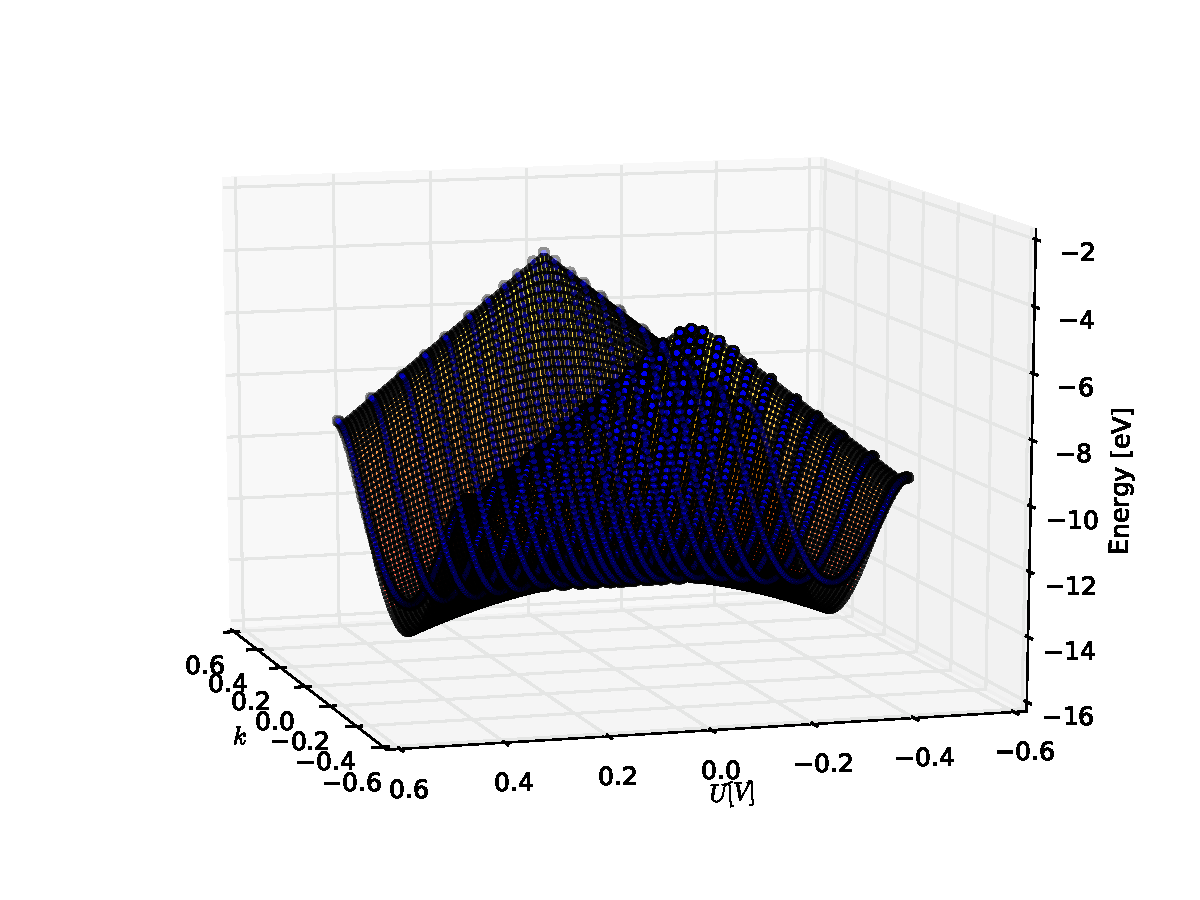
\includegraphics[width = 13cm]{Images/Hydrogen/charging/3D/figure_1-2}
	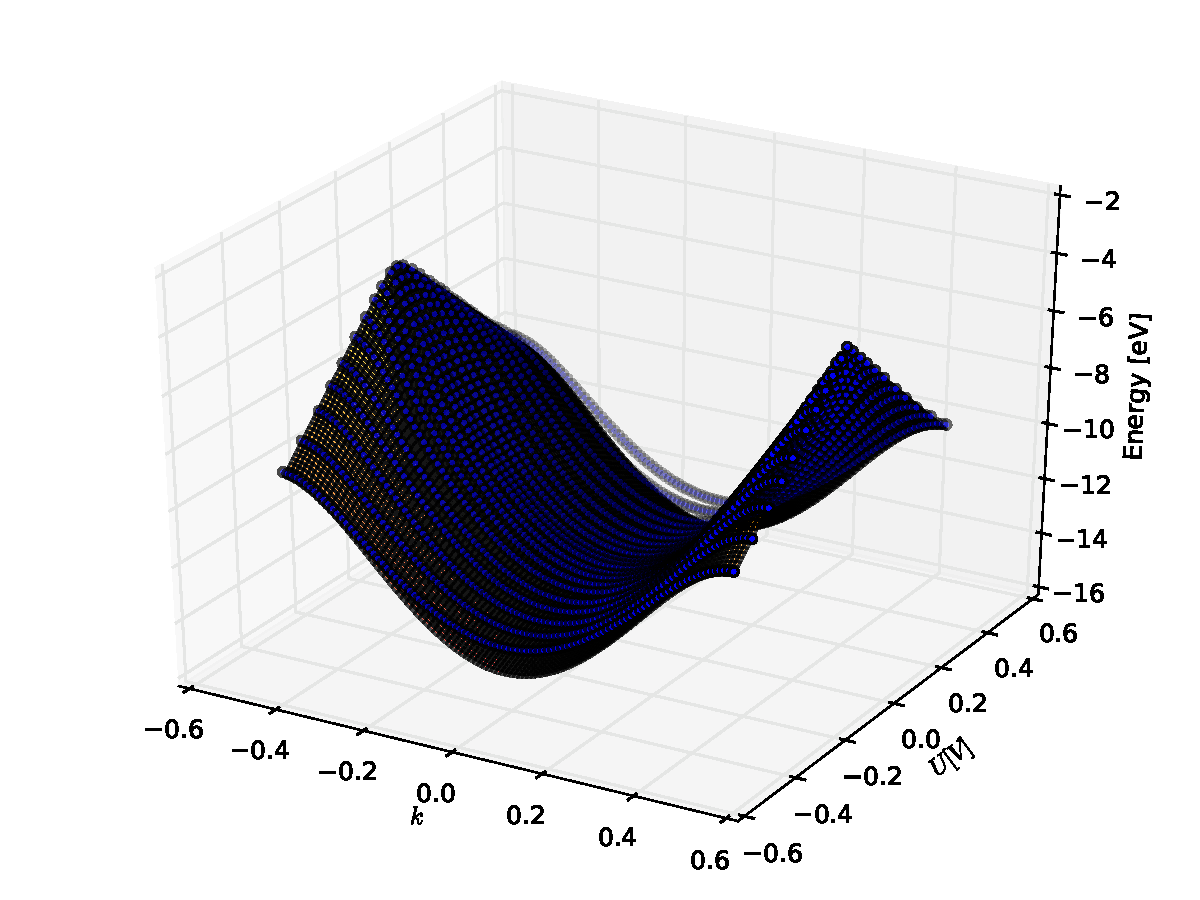
\includegraphics[width = 13cm]{Images/Hydrogen/charging/3D/figure_1-1}
	\caption{Band structure in respect to the cDFT potential $U$. Data points in blue and surface from fit.}
	\label{image_hydrogen_3D_2}
\end{figure}
\begin{figure}
	\centering
	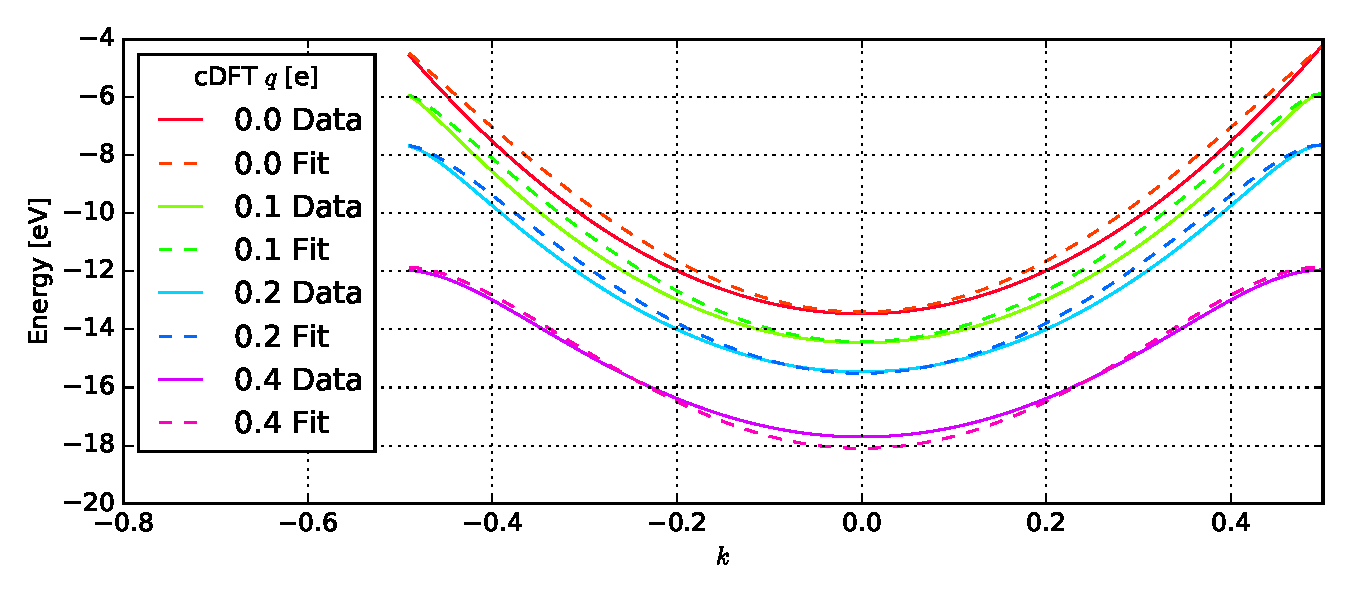
\includegraphics[width = 13cm]{Images/Hydrogen/charging/3D_cuts}
	\caption{Some slices of the band structure and fit for different displaced charges. The distance between the curves is manually increased for a better overview.}
	\label{image_hydrogen_3D_slices}
\end{figure}
\newpage To get rid of the $k$-dependency the average HOMO-band energy $E_\text{A}$ in respect to the external potential $V$ is calculated. A theoretical expression for this quantity can be found (derivation in the appendix, \cref{chapter_appendix}), namely:
\begin{align}
	E_\text{A}(V) &= \frac{-2}{N}\sum_k \left|E_k(V)\right|\\
				  &= \frac{-2}{\pi}\sqrt{V^2+4t_0^2}\int\limits_0^{\nicefrac{\pi}{2}}\dd\theta\ \sqrt{1-\xi^2\cdot\sin^2(\theta)}
				  \label{equation_elliptical_integral}
\end{align}
with $\xi^2 = \frac{4t_0^2-4\delta^2}{V^2+4t_0^2}$. The integral in \cref{equation_elliptical_integral} is known as the elliptical integral of the second kind and can be calculated numerically. With this expression it may be possible to obtain the hopping parameter $t_0$ through a fit to the average HOMO-band energy. To check this calculation for self-consistency a fit to some modelled data (data of the previous fit) is done. In \cref{image_hydrogen_homo_energy_charging} the data and fits can be seen, which already shows some mismatch between the calculated and modeled data from the earlier fit. It can be seen, that the modelled data is too big for a small external potential and too small for a big external potential. This tendency can also be seen by a close look at \cref{image_hydrogen_3D_slices}.\\
Nevertheless the data is fitted nicely and for the modelled data a value of $t_0 = \unit[4.6]{eV}$ is obtained, which is in perfect accordance to the previous result. From the real data a value of $t_0 = \unit[9.1]{eV}$ is obtained.\\
\begin{figure}[]
	\centering
	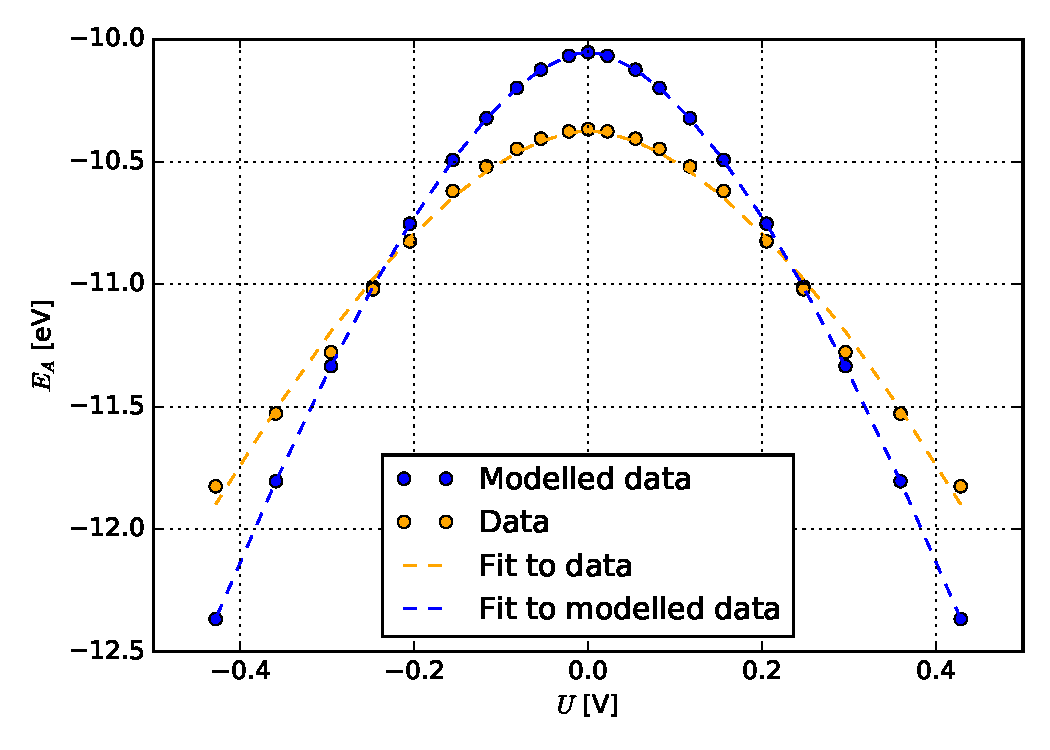
\includegraphics[width = 0.7\textwidth]{Images/Hydrogen/charging/Homo_energy_charge}
	\caption{Average HOMO-band energies in respect to the external potential $U$ with fits.}
	\label{image_hydrogen_homo_energy_charging}
\end{figure}
\begin{figure}[]
	\centering
	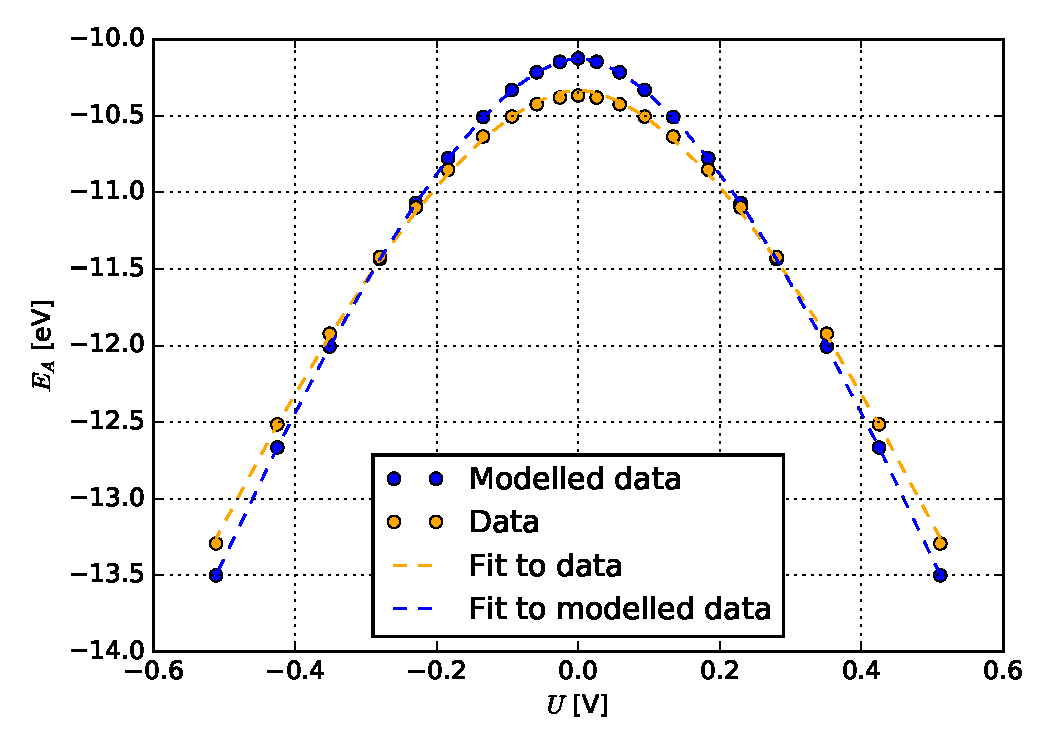
\includegraphics[width = 0.7\textwidth]{Images/Hydrogen/charging/Homo_energy_charge_sigma_32}
	\caption{Average HOMO-band energies in respect to the external potential $U$ with fits for $\sigma = \unit[0.32]{\AA}$.}
	\label{image_hydrogen_homo_energy_charging_sigma_32}
\end{figure}
Thus it can be concluded that at least for the hydrogen chain additional terms are needed to describe this phenomena correctly. For example, one may think of adding a \textsc{Hubbard} term to describe the electron-electron repulsion at the core positions or a term for next-nearest-neighbour-hopping \cite{PhysRevLett.103.067004,PhysRevB.82.155141}. Both would make the derivation of an analytical expression for the band energies more difficult and add new parameters, which should be determined in some other way.\\ In \cref{image_hydrogen_homo_energy_charging_sigma_32} the analogous data and fits to \cref{image_hydrogen_homo_energy_charging} for a $\sigma$ of $\unit[0.32]{\AA}$ can be seen. Here the fit to the data yields the hopping parameter $t_0 = \unit[6.1]{eV}$, which shows that the additional needed terms may have a $\sigma$-dependency or a less heuristic way of choosing the value for $\sigma$ may be found.\\
Since the general form of the band structure in respect to the displaced charge is still qualitatively well described and hydrogen often behaves a little tricky, this method is also tested for \emph{trans}-polyacetylene.
\subsection{Polyacetylene}
To use cDFT with polyacetylene different regions for charging have to be defined. Here two regions, each containing a CH-group, are chosen to make sure that the charge is transferred between those CH-groups and not between the carbon and hydrogen atoms (similar to \cref{image_region_gaussians}).\\
First the optimal value for $\sigma$ is calculated as before, namely by searching a value for $\sigma$, for which charge transport becomes the easiest (see \cref{image_sigmas_polyacetylene}). Here the value $\sigma = \unit[0.32]{\AA}$ is obtained and used for further calculations if not otherwise mentioned.\\
Next the band structure for different charge displacements is calculated (see \cref{image_polyacetylene_band_structure_charging}), which shows again the expected independence of the direction (sign) of the charge displacement. Also the expected band gap broadening and the systematic shift of the HOMO-band to lower energies can be seen for increasing charge displacements. Furthermore analogous effects in the same order of magnitude can be seen for all the other bands.\\
\begin{figure}[]
	\centering
	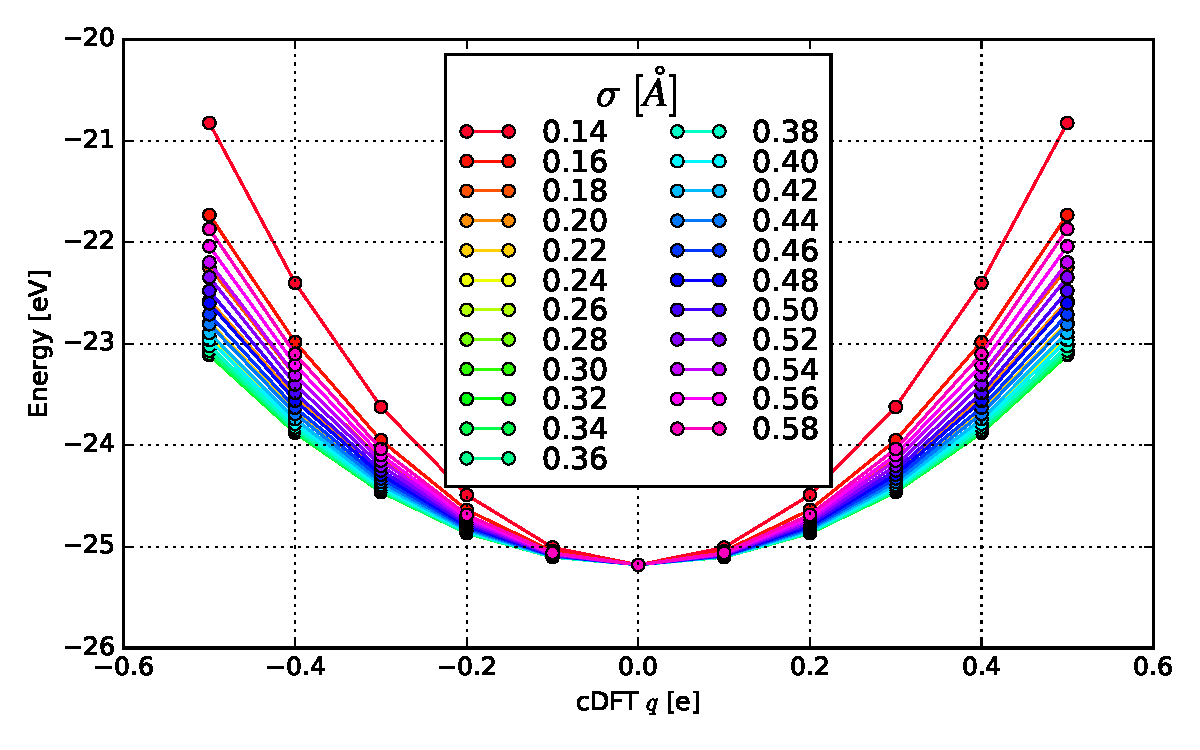
\includegraphics[width = 10cm]{Images/polyacetylene/charging/sigmas}
	\caption{Ground state energy of polyacetylene in respect to the displaced charge for different $\sigma$ of the \textsc{Gaussian} curves.}
	\label{image_sigmas_polyacetylene}
\end{figure}
\begin{figure}[!p]
	\centering
	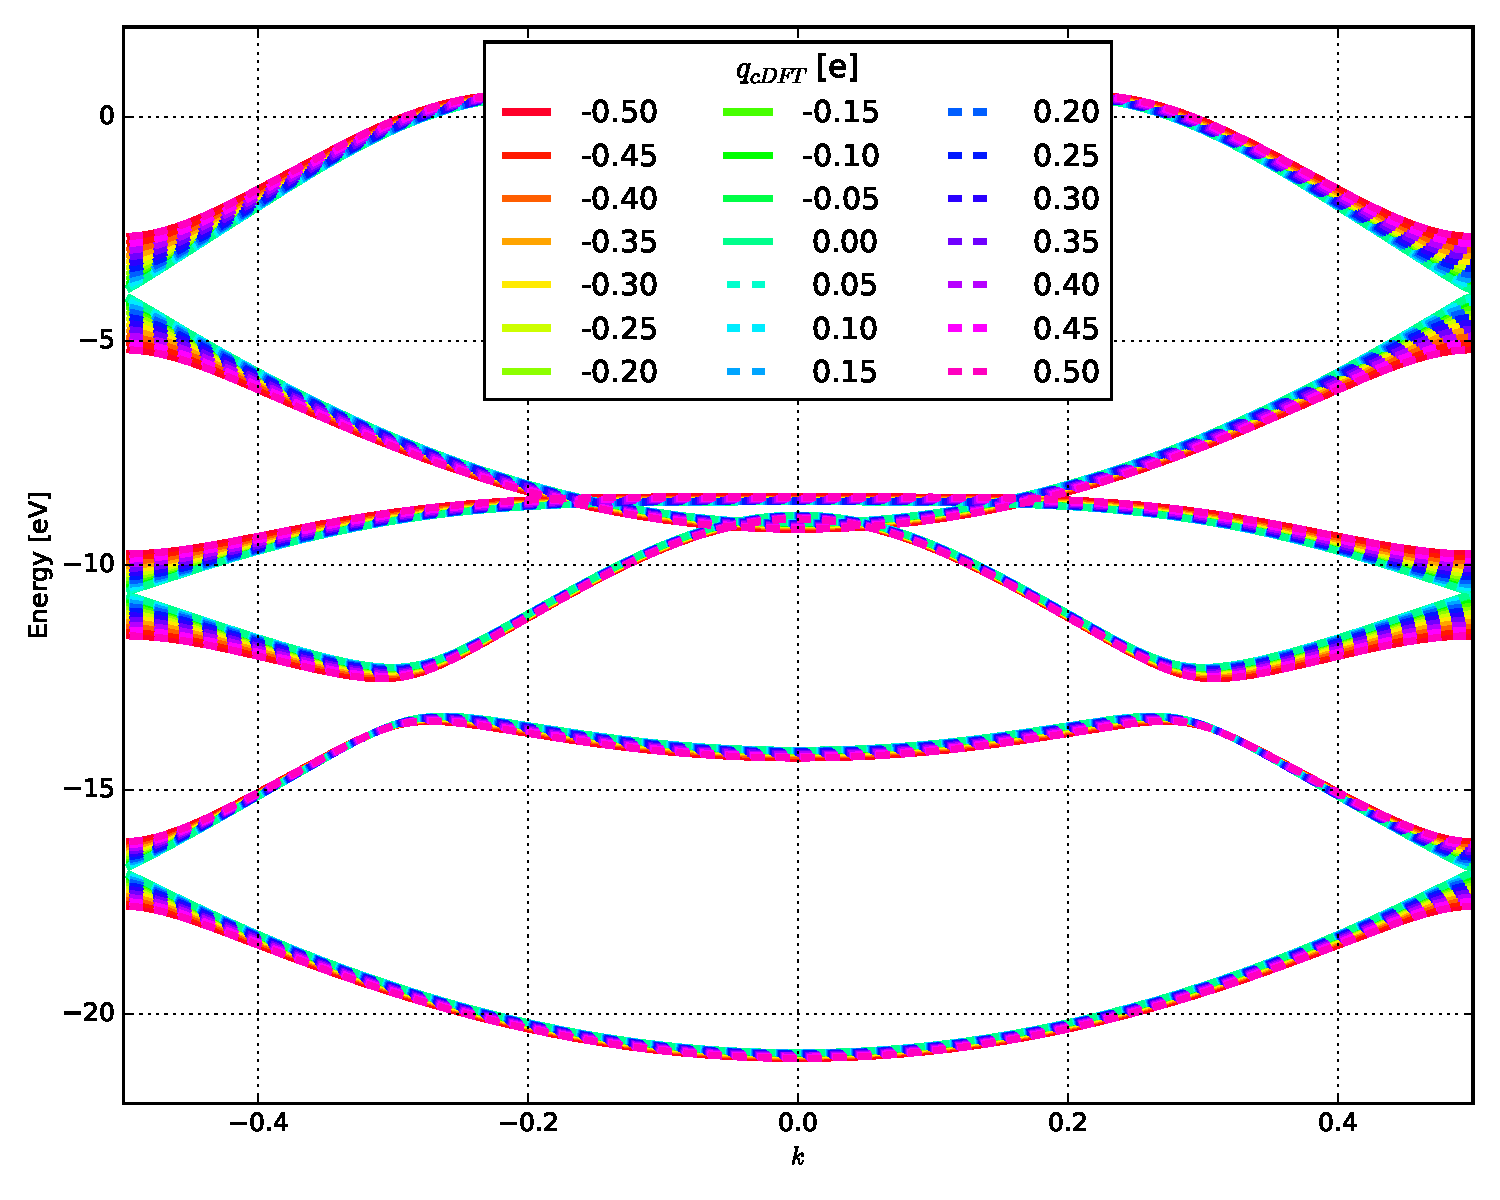
\includegraphics[width = 11cm]{Images/polyacetylene/charging/band_structure_q_1}
	\caption{Band structure of polyacetylene for different charge displacements. Here the five highest occupied bands and the LUMO-band are shown.}
	\label{image_polyacetylene_band_structure_charging}
\end{figure}
Also the antisymmetric behaviour of the HOMO- and LUMO-band in the outer regions, where no band interactions appear, can be seen, which matches the predictions of the calculated hopping eigenenergies:
\begin{align}
	E_k &= \pm \sqrt{V^2+\epsilon_k^2+\Delta_k^2}
\end{align}
In the next step the cDFT potentials $U_i$ are checked to show the expected antisymmetric behaviour $U_1 = -U_2$ for the different charge displacements. Here it is even more important than for the hydrogen chain to start from a neutral state and to use antisymmetric initial potentials (see \cref{image_polyacetylene_potentials_asymmetry}). In further calculations $U = \frac{1}{2}(U_1 - U_2)$ is used again as corresponding cDFT quantity to the energy variation $V$ at the even/odd positions from the model.\\
To calculate the proportionality factor between $U$ and $V$ the same method as for hydrogen is used, namely fitting the HOMO-band energies at the edge of the \textsc{Brillouin} zone to the predicted form:
\begin{align}
	E_\text{edge} &= -\sqrt{\left(cU\right)^2 + 4 \delta^2}
\end{align}
Due to the small, but not vanishing, distortion the additional term under the root is obtained. Thus a similar form of a negative absolute, but with a little rounding at the tip is expected. For the fit $\delta$ is fixed to a quarter of the earlier calculated band gap (\cref{table_summary_polyacetylene}), which yields a proportionality constant of $c = \unit[7.70]{e}$ (see \cref{image_border_energy_polyacetylene}).\\
\begin{figure}
	\centering
	\begin{subfigure}{0.45\textwidth}
	\centering
	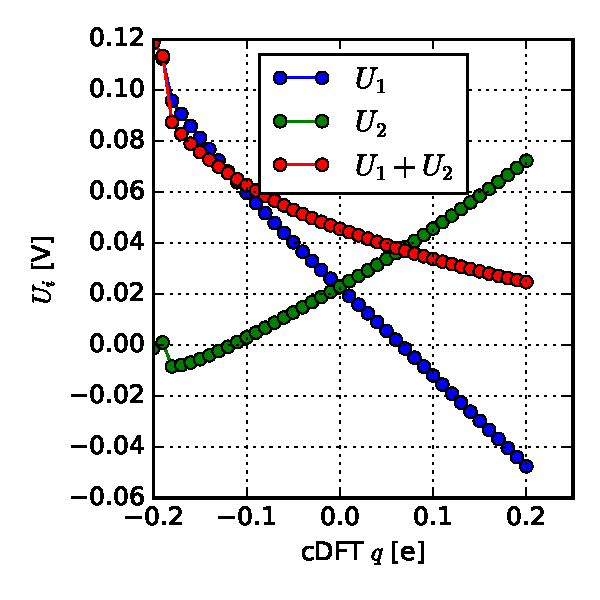
\includegraphics[width = \textwidth]{Images/polyacetylene/charging/potential_q_asymmetric}
	\caption{Symmetric initial cDFT potentials \mbox{$U_1 = U_2 > 0$} and order of charge displacement going from negative to  positive $q$.}
	\label{}
	\end{subfigure}\hspace*{.5cm}
	\begin{subfigure}{0.45\textwidth}
	\centering
	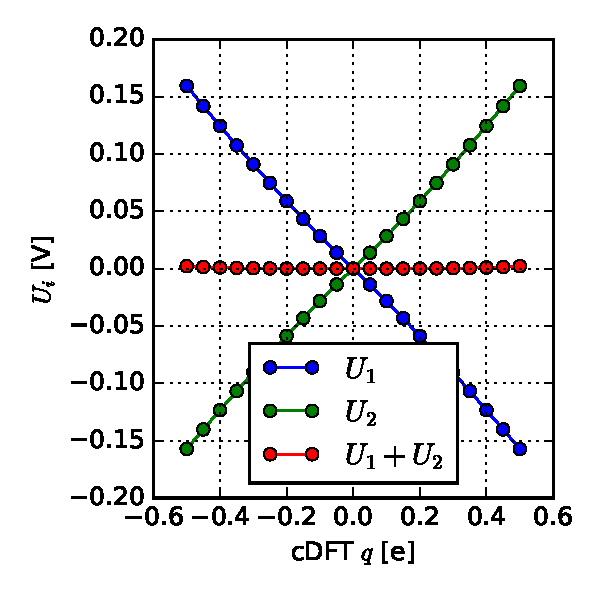
\includegraphics[width = \textwidth]{Images/polyacetylene/charging/potential_q_1}
	\caption{Asymmetric initial cDFT potentials $U_1 = -U_2$ and order of charge displacement going from neutral to  positive/negative $q$.}
	\label{}
	\end{subfigure}
	\caption{cDFT potentials $U_i$ in respect to the displaced charge for polyacetylene. The calculations are made for different orders of charging and different initial cDFT potentials.}
	\label{image_polyacetylene_potentials_asymmetry}
\end{figure}
\begin{figure}
	\centering
	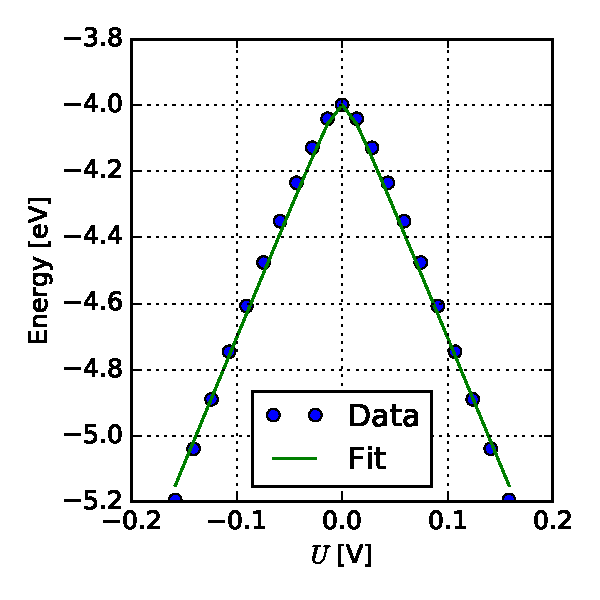
\includegraphics[width = 0.4\textwidth]{Images/polyacetylene/charging/border_energy_q_1}
	\caption{Homo-band energy at the edge of the \textsc{Brillouin} zone with fit for polyacetylene.}
	\label{image_border_energy_polyacetylene}
\end{figure}
For the further calculations the form of the HOMO-band without interactions has to be determined by taking corresponding contributions of the third, forth and fifth (HOMO) band. This data can then be fitted with the function (see \cref{image_polyacetylene_2D_fit}):
\begin{align}
	E(k, U) &= -\sqrt{\left(cU\right)^2 + \left(2t_0\cos(ka)\right)^2+\left(2\delta\sin(ka)\right)^2}
\end{align}
from which a value of $t_0 = \unit[2.6]{eV}$ is obtained, which matches the earlier calculated value perfectly. Furthermore it can be seen that the data is fitted very nicely. Also some slices of the 3D-plot in \cref{image_slices_polyacetylene} show the very good accordance of fit and data.\\
The average of the HOMO-band for the data and fit (modelled data) can be seen in \cref{image_HOMO_average_polyacetylene}, which match well, too. Also the data is fitted nicely by the expected form (see \cref{equation_elliptical_integral}). From the fit of the modelled data a perfect, self-consistent value of $t_0 = \unit[2.6]{eV}$ is obtained. The fit to the real data yields an also very good value of $t_0 = \unit[2.7]{eV}$.\\
Thus, a proof of principle is given that the hopping parameter $t_0$ for molecules, which are applicable for a description with the SSH-model, can be obtained by using cDFT charge displacement.\\
\newpage If the same procedure is done for \textsc{Gaussian} curves with $\sigma = \unit[0.24]{\AA}$, the average HOMO-band energies of the modelled and real data match much worse (see \cref{image_HOMO_average_polyacetylene_smaller_sigma}) and also a much worse hopping parameter of $t_0 = \unit[4.2]{\AA}$ is obtained. This shows that the heuristic way of choosing a value for $\sigma$ is at least for polyacetylene appropriate.\\
Since the first and second band and the third and forth band in \cref{image_polyacetylene_band_structure_charging} show some antisymmetric behaviour for charging and the calculation of the HOMO-band with no band interactions still needs some direct evaluation of the band structure a fit to the average energy of all five occupied bands, in the hope that influences of the lower bands cancel out, seems worth a try. In \cref{image_all_average_polyacetylene} this and the earlier calculated modelled data are shown. This yields a hopping parameter of $t_0 = \unit[1.7]{eV}$, which is a not too bad estimate and still leaves room for improvement.
\begin{figure}
	\centering
	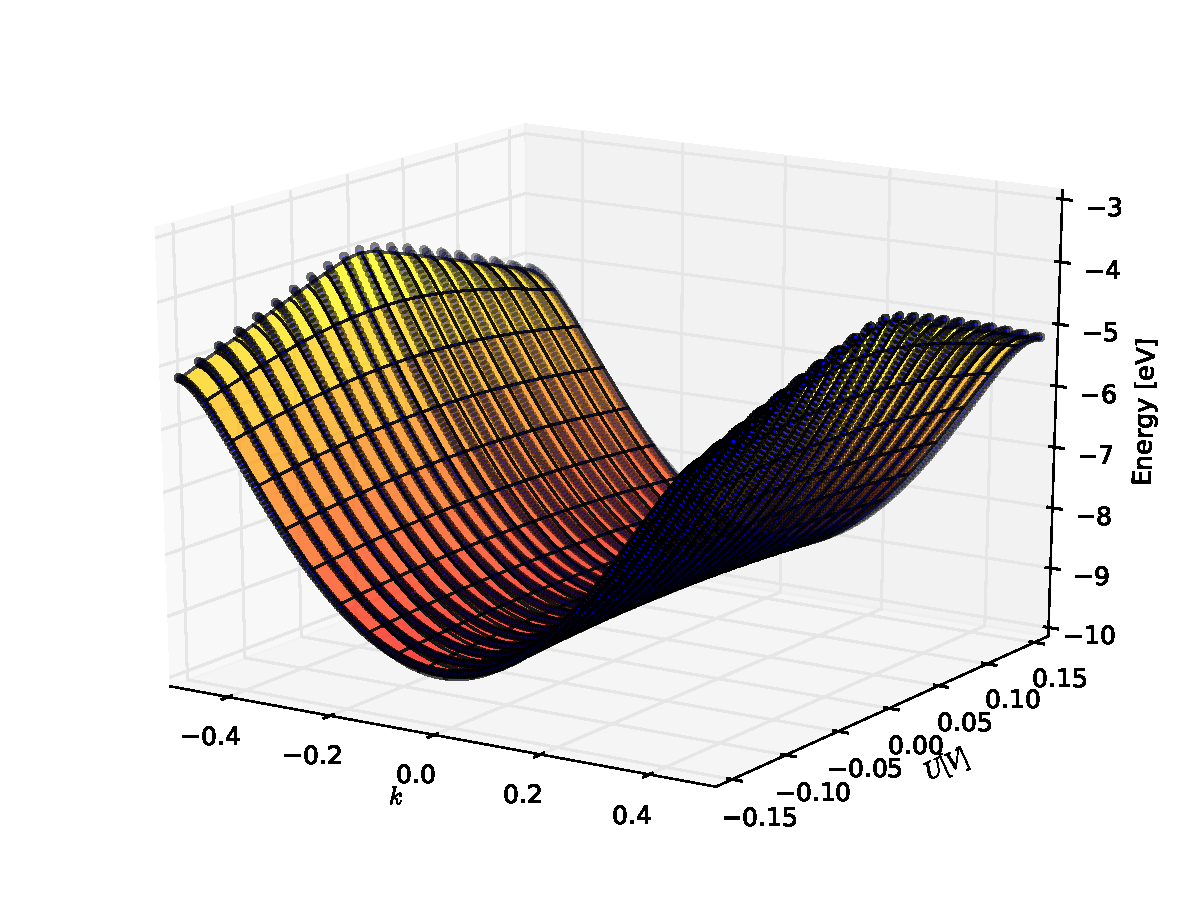
\includegraphics[width = 13cm]{Images/polyacetylene/charging/3D/figure_1-1}
	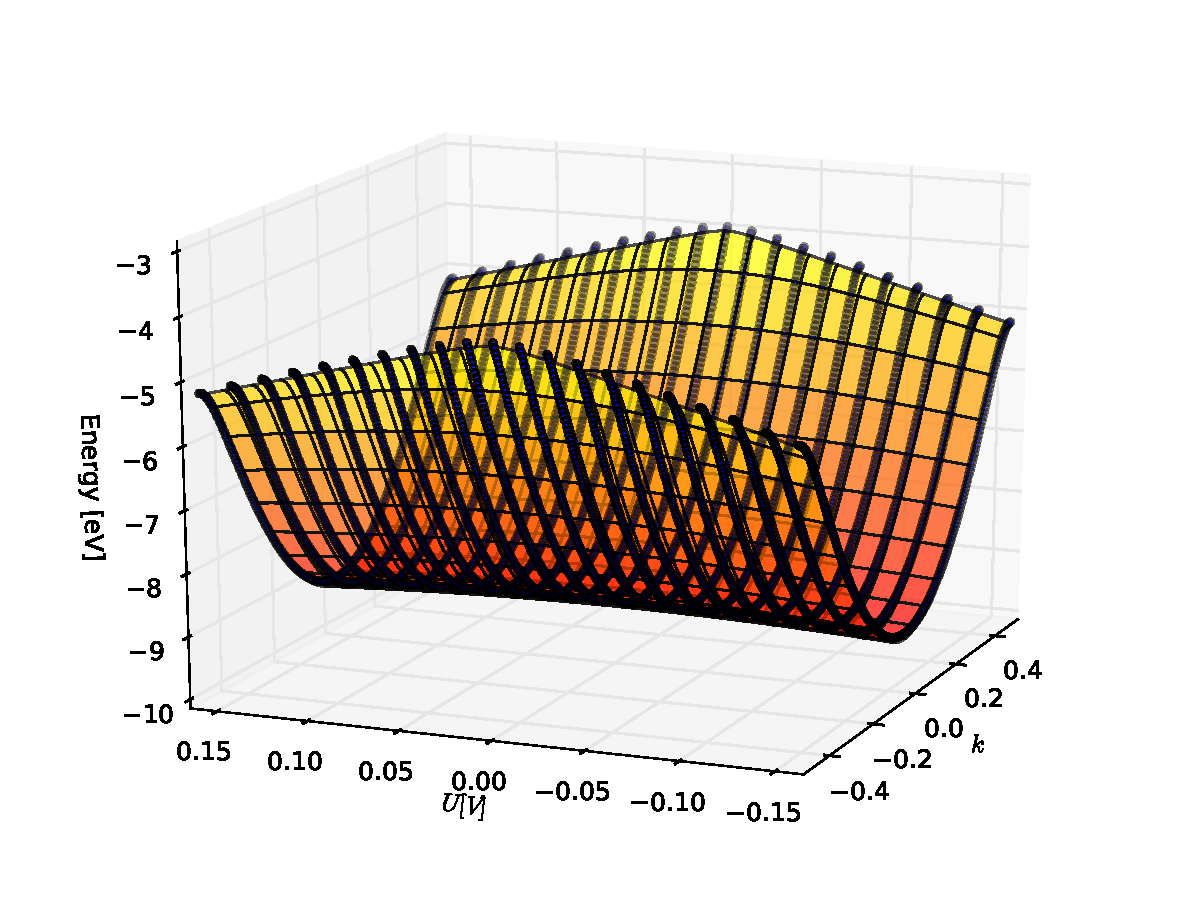
\includegraphics[width = 13cm]{Images/polyacetylene/charging/3D/figure_1-2}
	\caption{HOMO-band structure (for no band interactions) of polyacetylene in respect to the cDFT potential $U$. Data points in blue and surface from fit.}
	\label{image_polyacetylene_2D_fit}
\end{figure}
\begin{figure}
	\centering
	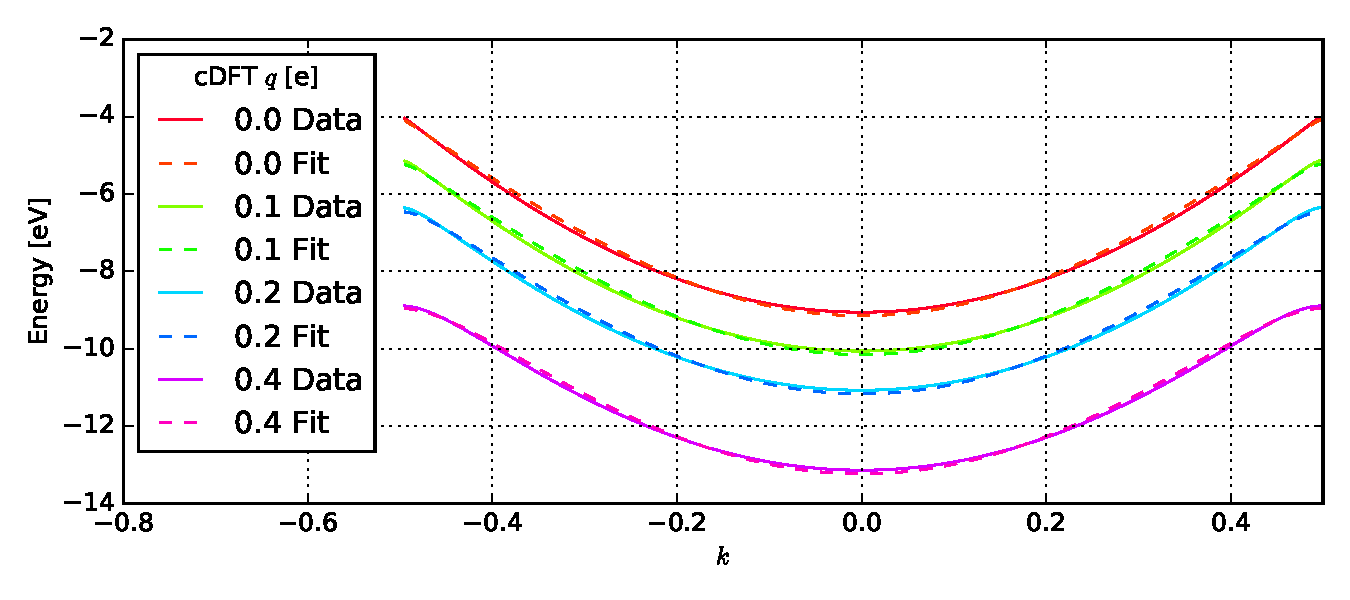
\includegraphics[width = 13cm]{Images/polyacetylene/charging/3D_cuts}
	\caption{Some slices of the band structure and fit  from polyacetylene for different displaced charges. The distance between the curves is manually increased for a better overview.}
	\label{image_slices_polyacetylene}
\end{figure}
\begin{figure}
	\centering
	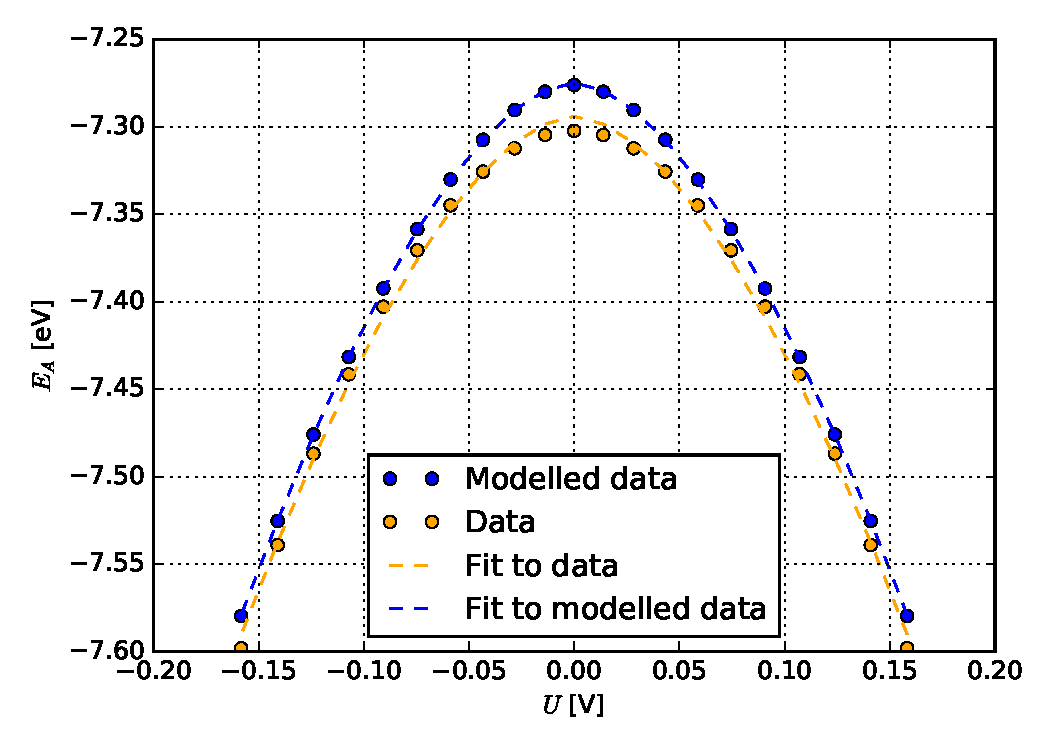
\includegraphics[width = 0.7\textwidth]{Images/polyacetylene/charging/Homo_energy_charge}
	\caption{Average HOMO-band energies of polyacetylene in respect to the external potential $U$ with fits.}
	\label{image_HOMO_average_polyacetylene}
\end{figure}
\begin{figure}
	\centering
	\includegraphics[width = .7\textwidth]{Images/polyacetylene/charging/Homo_energy_charge_smaller_sigma}
	\caption{Average HOMO-band energies of polyacetylene in respect to the external potential $U$ with fits for $\sigma = \unit[0.24]{\AA}$ of the \textsc{Gaussian} curves.}
	\label{image_HOMO_average_polyacetylene_smaller_sigma}
\end{figure}
\begin{figure}
	\centering
	\includegraphics[width = .7\textwidth]{Images/polyacetylene/charging/Band_energy_average_charge}
	\caption{Average energies of the five highest occupied bands of polyacetylene in respect to the external potential $U$. The modelled data from the HOMO-band is shown for comparison and thus the offsets are set to zero.}
	\label{image_all_average_polyacetylene}
\end{figure}
